%  A simple AAU report template.
%  2015-05-08 v. 1.2.0
%  Copyright 2010-2015 by Jesper Kjær Nielsen <jkn@es.aau.dk>
%
%  This is free software: you can redistribute it and/or modify
%  it under the terms of the GNU General Public License as published by
%  the Free Software Foundation, either version 3 of the License, or
%  (at your option) any later version.
%
%  This is distributed in the hope that it will be useful,
%  but WITHOUT ANY WARRANTY; without even the implied warranty of
%  MERCHANTABILITY or FITNESS FOR A PARTICULAR PURPOSE.  See the
%  GNU General Public License for more details.
%
%  You can find the GNU General Public License at <http://www.gnu.org/licenses/>.
%
%  A simple AAU report template.
%  2015-05-08 v. 1.2.0
%  Copyright 2010-2015 by Jesper Kjær Nielsen <jkn@es.aau.dk>
%
%  This is free software: you can redistribute it and/or modify
%  it under the terms of the GNU General Public License as published by
%  the Free Software Foundation, either version 3 of the License, or
%  (at your option) any later version.
%
%  This is distributed in the hope that it will be useful,
%  but WITHOUT ANY WARRANTY; without even the implied warranty of
%  MERCHANTABILITY or FITNESS FOR A PARTICULAR PURPOSE.  See the
%  GNU General Public License for more details.
%
%  You can find the GNU General Public License at <http://www.gnu.org/licenses/>.
%
\documentclass[11pt,twoside,a4paper,openright]{report}
%%%%%%%%%%%%%%%%%%%%%%%%%%%%%%%%%%%%%%%%%%%%%%%%
% Language, Encoding and Fonts
% http://en.wikibooks.org/wiki/LaTeX/Internationalization
%%%%%%%%%%%%%%%%%%%%%%%%%%%%%%%%%%%%%%%%%%%%%%%%
% Select encoding of your inputs. Depends on
% your operating system and its default input
% encoding. Typically, you should use
%   Linux  : utf8 (most modern Linux distributions)
%            latin1 
%   Windows: ansinew
%            latin1 (works in most cases)
%   Mac    : applemac
% Notice that you can manually change the input
% encoding of your files by selecting "save as"
% an select the desired input encoding. 
\usepackage[utf8]{inputenc}
% Make latex understand and use the typographic
% rules of the language used in the document.
\usepackage[english]{babel}
% Use the palatino font
\usepackage[sc]{mathpazo}
\linespread{1.05}         % Palatino needs more leading (space between lines)
% Choose the font encoding
\usepackage[T1]{fontenc}
%%%%%%%%%%%%%%%%%%%%%%%%%%%%%%%%%%%%%%%%%%%%%%%%
% Graphics and Tables
% http://en.wikibooks.org/wiki/LaTeX/Importing_Graphics
% http://en.wikibooks.org/wiki/LaTeX/Tables
% http://en.wikibooks.org/wiki/LaTeX/Colors
%%%%%%%%%%%%%%%%%%%%%%%%%%%%%%%%%%%%%%%%%%%%%%%%
% load a colour package
\usepackage{xcolor}
\definecolor{aaublue}{RGB}{33,26,82}% dark blue
% The standard graphics inclusion package
\usepackage{graphicx}
\graphicspath{ {figures/} }
% Set up how figure and table captions are displayed
\usepackage{caption}
\captionsetup{%
  font=footnotesize,% set font size to footnotesize
  labelfont=bf % bold label (e.g., Figure 3.2) font
}
% Make the standard latex tables look so much better
\usepackage{array,booktabs}
% Enable the use of frames around, e.g., theorems
% The framed package is used in the example environment
\usepackage{framed}

%%%%%%%%%%%%%%%%%%%%%%%%%%%%%%%%%%%%%%%%%%%%%%%%
% Mathematics
% http://en.wikibooks.org/wiki/LaTeX/Mathematics
%%%%%%%%%%%%%%%%%%%%%%%%%%%%%%%%%%%%%%%%%%%%%%%%
% Defines new environments such as equation,
% align and split 
\usepackage{amsmath}
% Adds new math symbols
\usepackage{amssymb}
% Use theorems in your document
% The ntheorem package is also used for the example environment
% When using thmmarks, amsmath must be an option as well. Otherwise \eqref doesn't work anymore.
\usepackage[framed,amsmath,thmmarks]{ntheorem}

%%%%%%%%%%%%%%%%%%%%%%%%%%%%%%%%%%%%%%%%%%%%%%%%
% Page Layout
% http://en.wikibooks.org/wiki/LaTeX/Page_Layout
%%%%%%%%%%%%%%%%%%%%%%%%%%%%%%%%%%%%%%%%%%%%%%%%
% Change margins, papersize, etc of the document
\usepackage[
  inner=28mm,% left margin on an odd page
  outer=41mm,% right margin on an odd page
  ]{geometry}
% Modify how \chapter, \section, etc. look
% The titlesec package is very configureable
\usepackage{titlesec}
\titleformat{\chapter}[display]{\normalfont\huge\bfseries}{\chaptertitlename\ \thechapter}{20pt}{\Huge}
\titleformat*{\section}{\normalfont\Large\bfseries}
\titleformat*{\subsection}{\normalfont\large\bfseries}
\titleformat*{\subsubsection}{\normalfont\normalsize\bfseries}
%\titleformat*{\paragraph}{\normalfont\normalsize\bfseries}
%\titleformat*{\subparagraph}{\normalfont\normalsize\bfseries}

% Clear empty pages between chapters
\let\origdoublepage\cleardoublepage
\newcommand{\clearemptydoublepage}{%
  \clearpage
  {\pagestyle{empty}\origdoublepage}%
}
\let\cleardoublepage\clearemptydoublepage

% Change the headers and footers
\usepackage{fancyhdr}
\pagestyle{fancy}
\fancyhf{} %delete everything
\renewcommand{\headrulewidth}{0pt} %remove the horizontal line in the header
\fancyhead[RE]{\small\nouppercase\leftmark} %even page - chapter title
\fancyhead[LO]{\small\nouppercase\rightmark} %uneven page - section title
\fancyhead[LE,RO]{\thepage} %page number on all pages
% Do not stretch the content of a page. Instead,
% insert white space at the bottom of the page
\raggedbottom
% Enable arithmetics with length. Useful when
% typesetting the layout.
\usepackage{calc}

%%%%%%%%%%%%%%%%%%%%%%%%%%%%%%%%%%%%%%%%%%%%%%%%
% Bibliography
% http://en.wikibooks.org/wiki/LaTeX/Bibliography_Management
%%%%%%%%%%%%%%%%%%%%%%%%%%%%%%%%%%%%%%%%%%%%%%%%
\usepackage[backend=bibtex,
  bibencoding=utf8
  ]{biblatex}
\addbibresource{bib/mybib}

%%%%%%%%%%%%%%%%%%%%%%%%%%%%%%%%%%%%%%%%%%%%%%%%
% Misc
%%%%%%%%%%%%%%%%%%%%%%%%%%%%%%%%%%%%%%%%%%%%%%%%
% Add bibliography and index to the table of
% contents
\usepackage[nottoc]{tocbibind}
% Add the command \pageref{LastPage} which refers to the
% page number of the last page
\usepackage{lastpage}
% Add todo notes in the margin of the document
\usepackage[
%  disable, %turn off todonotes
  colorinlistoftodos, %enable a coloured square in the list of todos
  textwidth=\marginparwidth, %set the width of the todonotes
  textsize=scriptsize, %size of the text in the todonotes
  ]{todonotes}

%%%%%%%%%%%%%%%%%%%%%%%%%%%%%%%%%%%%%%%%%%%%%%%%
% Hyperlinks
% http://en.wikibooks.org/wiki/LaTeX/Hyperlinks
%%%%%%%%%%%%%%%%%%%%%%%%%%%%%%%%%%%%%%%%%%%%%%%%
% Enable hyperlinks and insert info into the pdf
% file. Hypperref should be loaded as one of the 
% last packages
\usepackage{hyperref}
\hypersetup{%
	pdfpagelabels=true,%
	plainpages=false,%
	pdfauthor={Author(s)},%
	pdftitle={Title},%
	pdfsubject={Subject},%
	bookmarksnumbered=true,%
	colorlinks=false,%
	citecolor=black,%
	filecolor=black,%
	linkcolor=black,% you should probably change this to black before printing
	urlcolor=black,%
	pdfstartview=FitH%
}

\usepackage{graphicx}
\usepackage{amsmath}
\usepackage{listings}% package inclusion and set up of the document
% see, e.g., http://en.wikibooks.org/wiki/LaTeX/Formatting#Hyphenation
% for more information on word hyphenation
\hyphenation{ex-am-ple hy-phen-a-tion short}
\hyphenation{long la-tex}
% 
%  A simple AAU report template.
%  2015-05-08 v. 1.2.0
%  Copyright 2010-2015 by Jesper Kjær Nielsen <jkn@es.aau.dk>
%
%  This is free software: you can redistribute it and/or modify
%  it under the terms of the GNU General Public License as published by
%  the Free Software Foundation, either version 3 of the License, or
%  (at your option) any later version.
%
%  This is distributed in the hope that it will be useful,
%  but WITHOUT ANY WARRANTY; without even the implied warranty of
%  MERCHANTABILITY or FITNESS FOR A PARTICULAR PURPOSE.  See the
%  GNU General Public License for more details.
%
%  You can find the GNU General Public License at <http://www.gnu.org/licenses/>.
%
%
%
% see, e.g., http://en.wikibooks.org/wiki/LaTeX/Customizing_LaTeX#New_commands
% for more information on how to create macros

%%%%%%%%%%%%%%%%%%%%%%%%%%%%%%%%%%%%%%%%%%%%%%%%
% Macros for the titlepage
%%%%%%%%%%%%%%%%%%%%%%%%%%%%%%%%%%%%%%%%%%%%%%%%
%Creates the aau titlepage
\newcommand{\aautitlepage}[3]{%
  {
    %set up various length
    \ifx\titlepageleftcolumnwidth\undefined
      \newlength{\titlepageleftcolumnwidth}
      \newlength{\titlepagerightcolumnwidth}
    \fi
    \setlength{\titlepageleftcolumnwidth}{0.5\textwidth-\tabcolsep}
    \setlength{\titlepagerightcolumnwidth}{\textwidth-2\tabcolsep-\titlepageleftcolumnwidth}
    %create title page
    \thispagestyle{empty}
    \noindent%
    \begin{tabular}{@{}ll@{}}
      \parbox{\titlepageleftcolumnwidth}{
        \iflanguage{danish}{%
          
\includegraphics[width=\titlepageleftcolumnwidth]{figures/aau_logo_da}
        }{%
          
\includegraphics[width=\titlepageleftcolumnwidth]{figures/aau_logo_en}
        }
      } &
      \parbox{\titlepagerightcolumnwidth}{\raggedleft\sf\small
        #2
      }\bigskip\\
       #1 &
      \parbox[t]{\titlepagerightcolumnwidth}{%
      \textbf{Abstract:}\bigskip\par
        \fbox{\parbox{\titlepagerightcolumnwidth-2\fboxsep-2\fboxrule}{%
          #3
        }}
      }\\
    \end{tabular}
    \vfill
    \iflanguage{danish}{%
      \noindent{\footnotesize\emph{Rapportens indhold er frit tilgængeligt, men offentliggørelse (med kildeangivelse) må kun ske efter aftale med forfatterne.}}
    }{%
      \noindent{\footnotesize\emph{The content of this report is freely available, but publication (with reference) may only be pursued due to agreement with the author.}}
    }
    \clearpage
  }
}

%Create english project info
\newcommand{\englishprojectinfo}[8]{%
  \parbox[t]{\titlepageleftcolumnwidth}{
    \textbf{Title:}\\ #1\bigskip\par
    \textbf{Theme:}\\ #2\bigskip\par
    \textbf{Project Period:}\\ #3\bigskip\par
    \textbf{Project Group:}\\ #4\bigskip\par
    \textbf{Participant(s):}\\ #5\bigskip\par
    \textbf{Supervisor(s):}\\ #6\bigskip\par
    \textbf{Copies:} #7\bigskip\par
    \textbf{Page Numbers:} \pageref{LastPage}\bigskip\par
    \textbf{Date of Completion:}\\ #8
  }
}

%Create danish project info
\newcommand{\danishprojectinfo}[8]{%
  \parbox[t]{\titlepageleftcolumnwidth}{
    \textbf{Titel:}\\ #1\bigskip\par
    \textbf{Tema:}\\ #2\bigskip\par
    \textbf{Projektperiode:}\\ #3\bigskip\par
    \textbf{Projektgruppe:}\\ #4\bigskip\par
    \textbf{Deltager(e):}\\ #5\bigskip\par
    \textbf{Vejleder(e):}\\ #6\bigskip\par
    \textbf{Oplagstal:} #7\bigskip\par
    \textbf{Sidetal:} \pageref{LastPage}\bigskip\par
    \textbf{Afleveringsdato:}\\ #8
  }
}

%%%%%%%%%%%%%%%%%%%%%%%%%%%%%%%%%%%%%%%%%%%%%%%%
% An example environment
%%%%%%%%%%%%%%%%%%%%%%%%%%%%%%%%%%%%%%%%%%%%%%%%
\theoremheaderfont{\normalfont\bfseries}
\theorembodyfont{\normalfont}
\theoremstyle{break}
\def\theoremframecommand{{\color{gray!50}\vrule width 5pt \hspace{5pt}}}
\newshadedtheorem{exa}{Example}[chapter]
\newenvironment{example}[1]{%
		\begin{exa}[#1]
}{%
		\end{exa}
}
% my new macros

\begin{document}
%frontmatter
\pagestyle{empty} %disable headers and footers
\pagenumbering{roman} %use roman page numbering in the frontmatter
%  A simple AAU report template.
%  2015-05-08 v. 1.2.0
%  Copyright 2010-2015 by Jesper Kjær Nielsen <jkn@es.aau.dk>
%
%  This is free software: you can redistribute it and/or modify
%  it under the terms of the GNU General Public License as published by
%  the Free Software Foundation, either version 3 of the License, or
%  (at your option) any later version.
%
%  This is distributed in the hope that it will be useful,
%  but WITHOUT ANY WARRANTY; without even the implied warranty of
%  MERCHANTABILITY or FITNESS FOR A PARTICULAR PURPOSE.  See the
%  GNU General Public License for more details.
%
%  You can find the GNU General Public License at <http://www.gnu.org/licenses/>.
%
\pdfbookmark[0]{Front page}{label:frontpage}%
\begin{titlepage}
  \addtolength{\hoffset}{0.5\evensidemargin-0.5\oddsidemargin} %set equal margins on the frontpage - remove this line if you want default margins
  \noindent%
  \begin{tabular}{@{}p{\textwidth}@{}}
    \toprule[2pt]
    \midrule
    \vspace{0.2cm}
    \begin{center}
    \Huge{\textbf{
      Differential Drive Robot with Obstacle Avoidance% insert your title here
    }}
    \end{center}
    \begin{center}
      \Large{
        - Subtitle -% insert your subtitle here
      }
    \end{center}
    \vspace{0.2cm}\\
    \midrule
    \toprule[2pt]
  \end{tabular}
  \vspace{4 cm}
  \begin{center}
    {\large
      Project Report%Insert document type (e.g., Project Report)
    }\\
    \vspace{0.2cm}
    {\Large
      Group Name/Number%Insert your group name or real names here
    }
  \end{center}
  \vfill
  \begin{center}
  Aalborg University\\
  Electronics and IT
  \end{center}
\end{titlepage}
\clearpage

\thispagestyle{empty}
{\small
\strut\vfill % push the content to the bottom of the page
\noindent Copyright \copyright{} Aalborg University 2015\par
\vspace{0.2cm}
\noindent Here you can write something about which tools and software you have used for typesetting the document, running simulations and creating figures. If you do not know what to write, either leave this page blank or have a look at the colophon in some of your books.
}
\clearpage


\pdfbookmark[0]{English title page}{label:titlepage_en}
\aautitlepage{%
  \englishprojectinfo{
    Obstacle Avoidance for a Differential Drive Robot %title
  }{%
    Automation %theme
  }{%
    Fall Semester 2016 %project period
  }{%
    ED5-8 % project group
  }{%
    %list of group members
    Philip Philev\\ 
    Mihkel Soolep\\
    
  }{%
    %list of supervisors
    Simon Pedersen\\
    
  }{%
    0 % number of printed copies
  }{%
    \today % date of completion
  }%
}{%department and address
  \textbf{Electronics and IT}\\
  Aalborg University\\
  \href{http://www.aau.dk}{http://www.aau.dk}
}{% the abstract
  The rising development in automation has lead to the almost unprecedented surge of electric autonomous vehicles. To better understand the technologies used in the fields of autonomous vehicles and the smaller scale mobile robotics, this project was carried out.
A model describing and analysing the behaviour of a differential drive robot was created, alongside a theoretical PID controller. 
The application was conducted on a described set of hardware, which was later programmed using the Raspberry Pi platform. The development process includes basic software and leads to the implementation of obstacle avoidance 
 
}


\cleardoublepage
\pdfbookmark[0]{Contents}{label:contents}
\pagestyle{fancy} %enable headers and footers again
\tableofcontents
\chapter*{Preface\markboth{Preface}{Preface}}\label{ch:preface}
\addcontentsline{toc}{chapter}{Preface}
Here is the preface. You should put your signatures at the end of the preface.

\vspace{\baselineskip}\hfill Aalborg University, \today
\vfill\noindent
\begin{minipage}[b]{0.45\textwidth}
 \centering
 \rule{\textwidth}{0.5pt}\\
  Philip Philev\\
 {\footnotesize <pphile14@student.aau.dk>}
\end{minipage}
\hfill
\begin{minipage}[b]{0.45\textwidth}
 \centering
 \rule{\textwidth}{0.5pt}\\
  Mihkel Soolep\\
 {\footnotesize <username2@XX.aau.dk>}
\end{minipage}
\vspace{3\baselineskip}


\cleardoublepage
%mainmatter
\pagenumbering{arabic} %use arabic page numbering in the mainmatter
\chapter{Introduction}\label{ch:introduction}

\paragraph{The Future of Vehicle Automation} 

In recent years, a big emphasis has been put on the development of autonomous or semi-autonomous ground vehicles. It comes as no surprise considering it is no longer a question of \textit{will} this technology be implemented, but rather \textit{when}.The benefits of autonomous vehicle integration can be considered invaluable. Currently 90\% of motor vehicle fatalities are estimated to be due to human errors, meaning that vehicle automation could result in substantial decrease of accidents. Furthermore, depending on the percentage of autonomous vehicles on the roads, a research concluded, a drastic reduction in traffic and congestions .\cite{DriverlessCar}

Nonetheless, there is still much work to be done in perfecting the control as well as the sensing capabilities of autonomous ground vehicles, if they are to become the default means of automotive transportation. Some of the issues consist of environmental conditions, which may disturb the sensors accuracy; precise mapping awareness, such as live maps that update when there is ongoing maintenance of infrastructure etc.; improved sensing capabilities (e.g advanced lidars) that can differentiate road damage, liquid spills etc.; ethical choices (as when an accident cannot be avoided), choosing to minimize potential damage and avoid casualties.\cite{DriverlessCar}

\subparagraph{Levels of Automation} 

Automated vehicles, as defined by the \textit{National Highway Traffic Safety Administration}(NHTSA - USA), are ones in which at least some aspects of a safety-critical control function occurs without the operator's direct input.(e.g steering, throttle,braking etc.)As such they are classified by the \textbf{NHTSA} in five levels:\cite{NHTSA}

\begin{itemize}

\item \textbf{Level 0 - No Automation} \\
Logically, this level does not include any direct automation functions, however it may include some warning systems such as blind spot monitoring. The operator has the complete control over the vehicle. 
\item \textbf{Level 1 - Function Specific Automation} \\
The system may utilize one or more control functions operating independently from each other, such as cruise control or dynamic brake support. Nevertheless the driver has over control and can limit the functions of the supported aid systems.
\item \textbf{Level 2 - Combined Function Automation} \\
The system utilizes at least two primary control functions, intercommunicating with each other in order to allow the operator's disengagement from physical operation of the vehicle. An example of such is a combination between \textit{adaptive cruise control} and \textit{lane centering}. The driver is still responsible for monitoring the environment, even when automated operating mode is enabled.
\item \textbf{Level 3 - Limited Self-Driving Automation} \\
The driver accepts to cede full control of all safety-critical functions under certain conditions, and rely completely on the vehicle to monitor the environment if a transition toward manual control is required. Such level of control is observed in automated or self-driving vehicles that conclude when the system is unable to handle an environment, such as road construction site, requiring specific manoeuvres. The driver is not expected to fully pay attention to the road, but is advised to pay attention to sudden changes.
\item \textbf{Level 4 - Full Self-Driving Automation} \\
Vehicle is designed to solely operate all safety-critical functions and supervise road conditions. Apart from providing destination input, the driver is not expected to maintain control at any point of the trip.
  
\end{itemize}

Currently \textbf{Level 4} automation is in active development stage, which means it won't be long until every newly manufactured vehicle has an above level 1 degree of automation.\cite{NHTSA}

\section{Mobile robotics}

While autonomous cars are becoming closer to "computer on wheels" rather than mechanical cars, as Elon Musk said in an interview, mobile robots could be viewed as the harbinger of this new era of automation.\cite{ElonMusk} Most systems, present in autonomous cars, are a scaled-up version of what has been present in robotics for a considerate time. Furthermore, an error or a failure of a system in an autonomous car would have much larger consequences than a system failure in domestic cleaning robot per se.
That is why, the general motivation for this project has been to model, analyse and develop a wheeled mobile robot, resulting in knowledge that could later be applied in the more "mature" industry of autonomous vehicles. 

\section{Motivation and summary of project}
This paper is concerned with the development of a feedback control and obstacle avoidance in a differential drive robot. The information is distributed in five chapter, which individually cover most of the information needed to recreate the results obtained in this paper. Further development would increase the accuracy of developed model, as well as the physical system.    
\chapter{Hardware}\label{ch:hardware}


In the following chapter the hardware used to create the robot is discussed.
The first decision made was what platform to use, based on the available resources and knowledge of use.

\section{Single board computer} 

The Raspberry Pi is the platform of choice used in the development of this project. Several factors influenced the choice, the most prominent of which was the familiarity the single board computer offered. Previous usage of Raspberry Pi 2B, allowed for faster decision making, when exploring for potential resources. 

\begin{figure}[h]
\centering
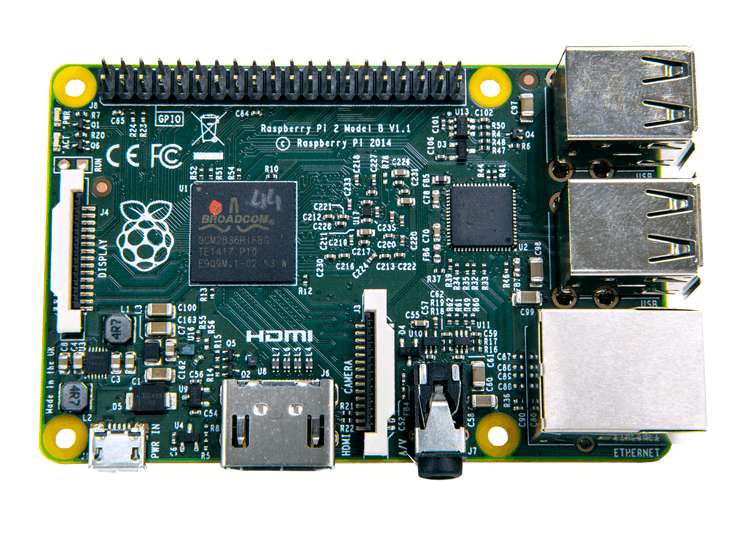
\includegraphics[width = 0.4\textwidth]{Raspberry-Pi-2}
\caption{Raspberry Pi 2B}
\label{fig::rasppi2b}
\end{figure}

\begin{figure}[h]
\centering
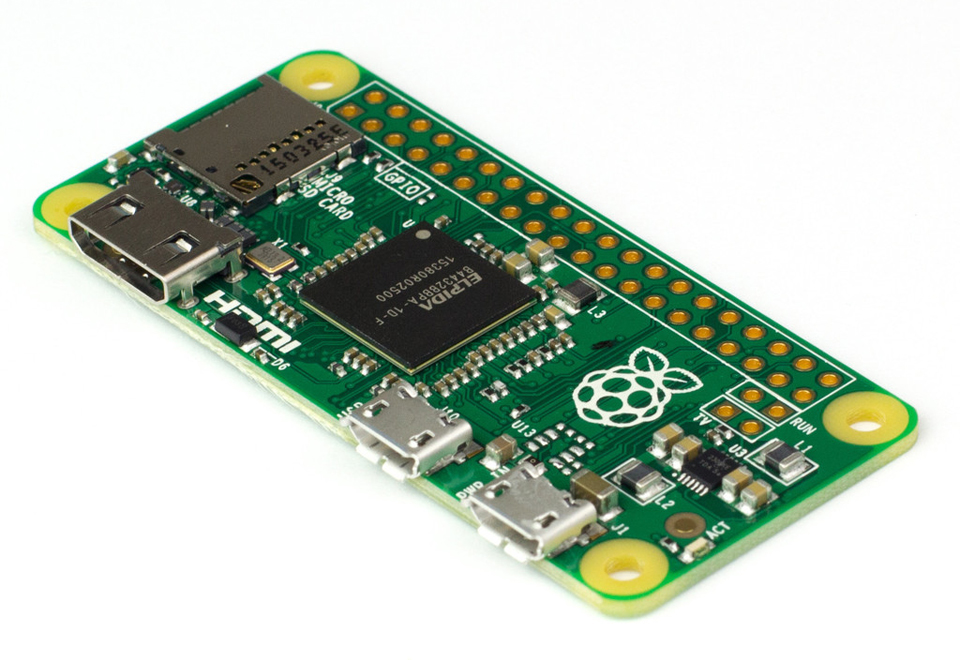
\includegraphics[width = 0.4\textwidth]{raspberry_pi_zero_1}
\caption{Raspberry Pi Zero}
\label{fig::raspizero}
\end{figure}

The initial choice was a Raspberry Pi 2B, however, after consideration of the size and required power consumption, a choice was made to use Raspberry Pi Zero instead.  

Performance of the two computers is almost similar, with the exception that the Zero model has less RAM compared to its 2B counterpart. Nevertheless, no significant impact was registered.

Specs of the Raspberry Pi Zero:
1Ghz, Single-core CPU
512MB RAM
Mini HDMI and USB On-The-Go ports
Micro USB power
HAT-compatible 40-pin header
Composite video and reset headers

\section{Distance measuring} 

Since the main purpose of the device would be to avoid obstacles, distance measuring sensors are required. There are several choices when it comes to distance sensors, vastly ranging in price and accuracy. The optimal choice would be a Lidar, however, at the time of development of this paper, the prices for Lidar were to high for practical implementation in a consumer application. 
As a result, the choice was made to use a set of ultrasonic sensors, which scaled well according to price and accuracy of measurements.
Three HC-SR04 ultrasonic sensors were used for distance measuring purposes in the device. The positioning of the sensors is on the front, and on the sides.

\begin{figure}[h]
\centering
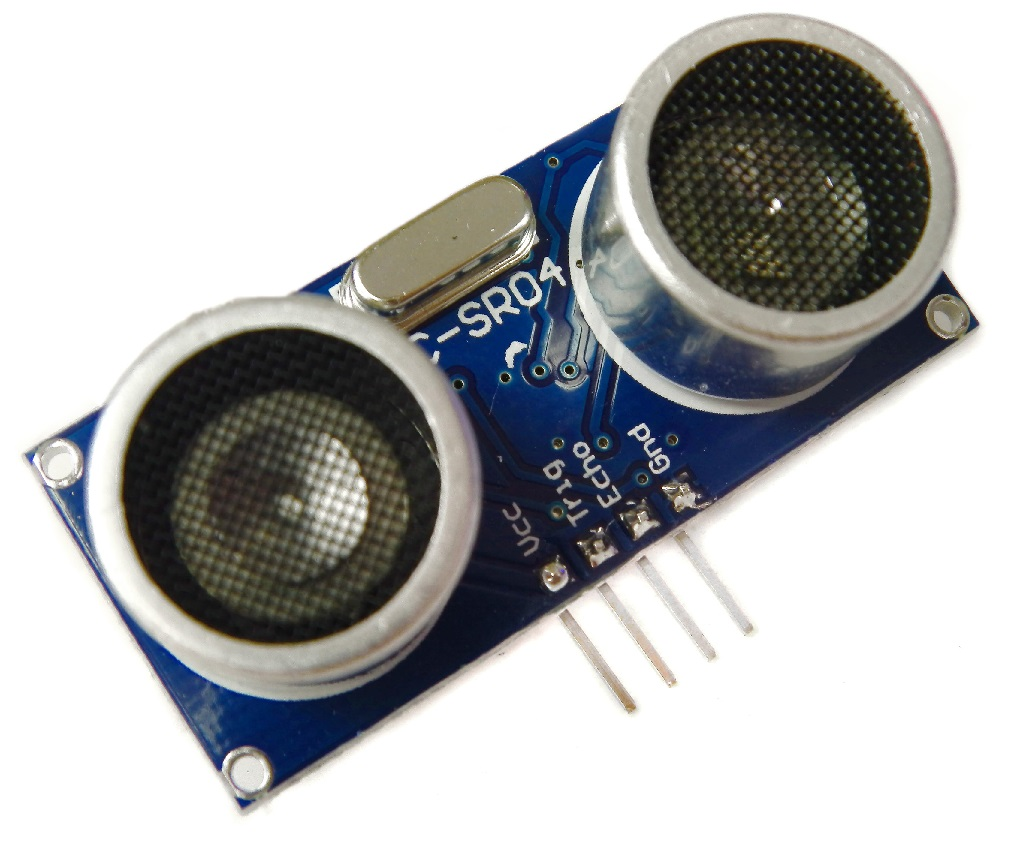
\includegraphics[width = 0.4\textwidth]{hc-sr04}
\caption{Ultra sonic sensor HC-SR04}
\label{fig::hcsr04}
\end{figure}

\section{DC motors and chassis} 

Considering the body of the robot, an inexpensive set of DC motors with a chassis was purchased and assembled. It comes with an attachable tachometer wheel for the motor, in order to incorporate a rotary encoder in the design, crucial for regulating the speed of the individual wheels.\cite{Motorref}

\begin{figure}[h]
\centering
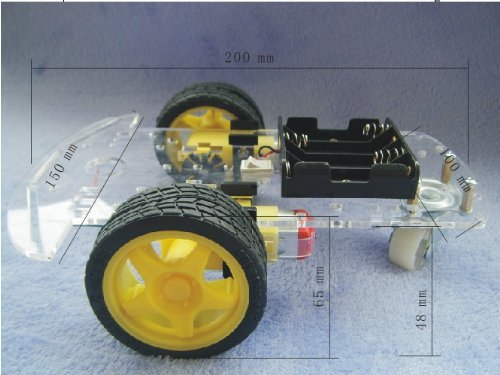
\includegraphics[width = 0.4\textwidth]{chassie}
\caption{Chassie and the two DC motors with a power supply}
\label{fig::chassie}
\end{figure}

Motor specs:

Voltage:
DC 3V
DC 5V
DC 6V
Current:
100 MA
100MA
120MA
Reduction rate:48:1
RPM (With tire):100,190,240
Tire Diameter:66mm
Car Speed(M/minute):20,39,48

Motor Weight (g):50

Motor Size:70mm*22mm*18mm

Noise:<65dB 

The two motors are identical and are used to move, as well as steer, the device and to 

\section{Motor driver} 

At the beginning of the project a L9110S DC Stepper Motor Driver H-Bridge was used, capable of controlling the direction of rotation of the wheels, but it was soon discovered the suggested driver was not capable of regulating the motor speeds.
To control the speed of the robot, a replacement with a L298N driver had to be performed.
The second driver was capable of using the PWM to regulate the speed of the motors.

\begin{figure}[h]
\centering
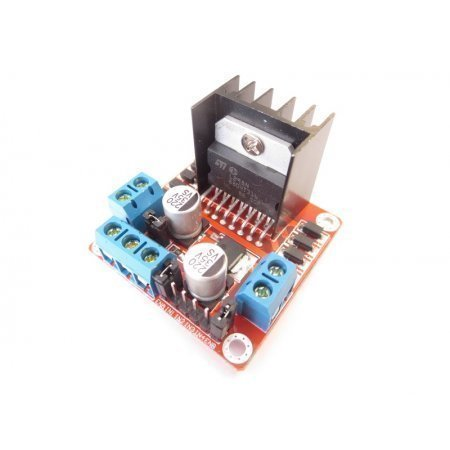
\includegraphics[width = 0.4\textwidth]{driver2}
\caption{The L298N driver}
\label{fig::driver2}
\end{figure}

Driver specs:
Working mode:	H bridge (double lines)
Control chip:	L298N (ST)
Logical voltage:	5V
Driving voltage:	5V-35V
Logical current:	max 36mA
Driving current:	2A (max single bridge)
Maximum power:	25W
Storage temperature:	-20 C +135 C
Periphery dimension:	43 x 43 x 27mm(L x W x H)

\section{Speed sensor}

The speed of the wheels is measured by the LM393 IR speed sensors attached to the tachometer wheel of the motor.\cite{SpeedSensor}

\begin{figure}[h]
\centering
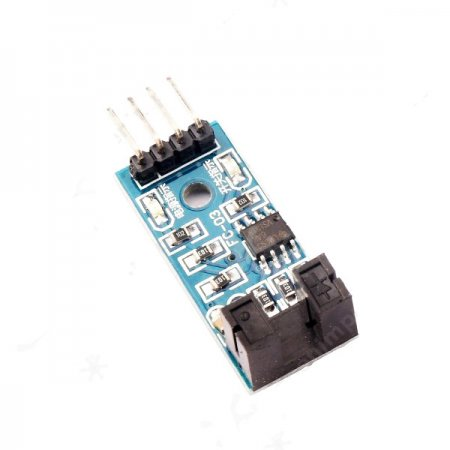
\includegraphics[width = 0.4\textwidth]{irspeed}
\caption{The LM393 IR speed sensor}
\label{fig::driver2}
\end{figure}

The speed sensor is used to estimate the error of the wheel speed.
Features:

Working voltage: 3.3V~5V
Weight: 8g
Dimensions: Approx.3.2 x 1.4 x 0.7cm
5mm Groove width
Using wide voltage LM393 comparator
Application: Widely used in dynamo speed detecting, pulse counting, etc
Output form: Digital switch output (0 and 1) and Analog for Sensitivity.


\section{Wi-Fi adapter}

In order to perform wireless monitoring, as well as extend the connectivity, an Edimax EW-7811Un Wi-Fi adapter, was used. 

\begin{figure}[h]
\centering
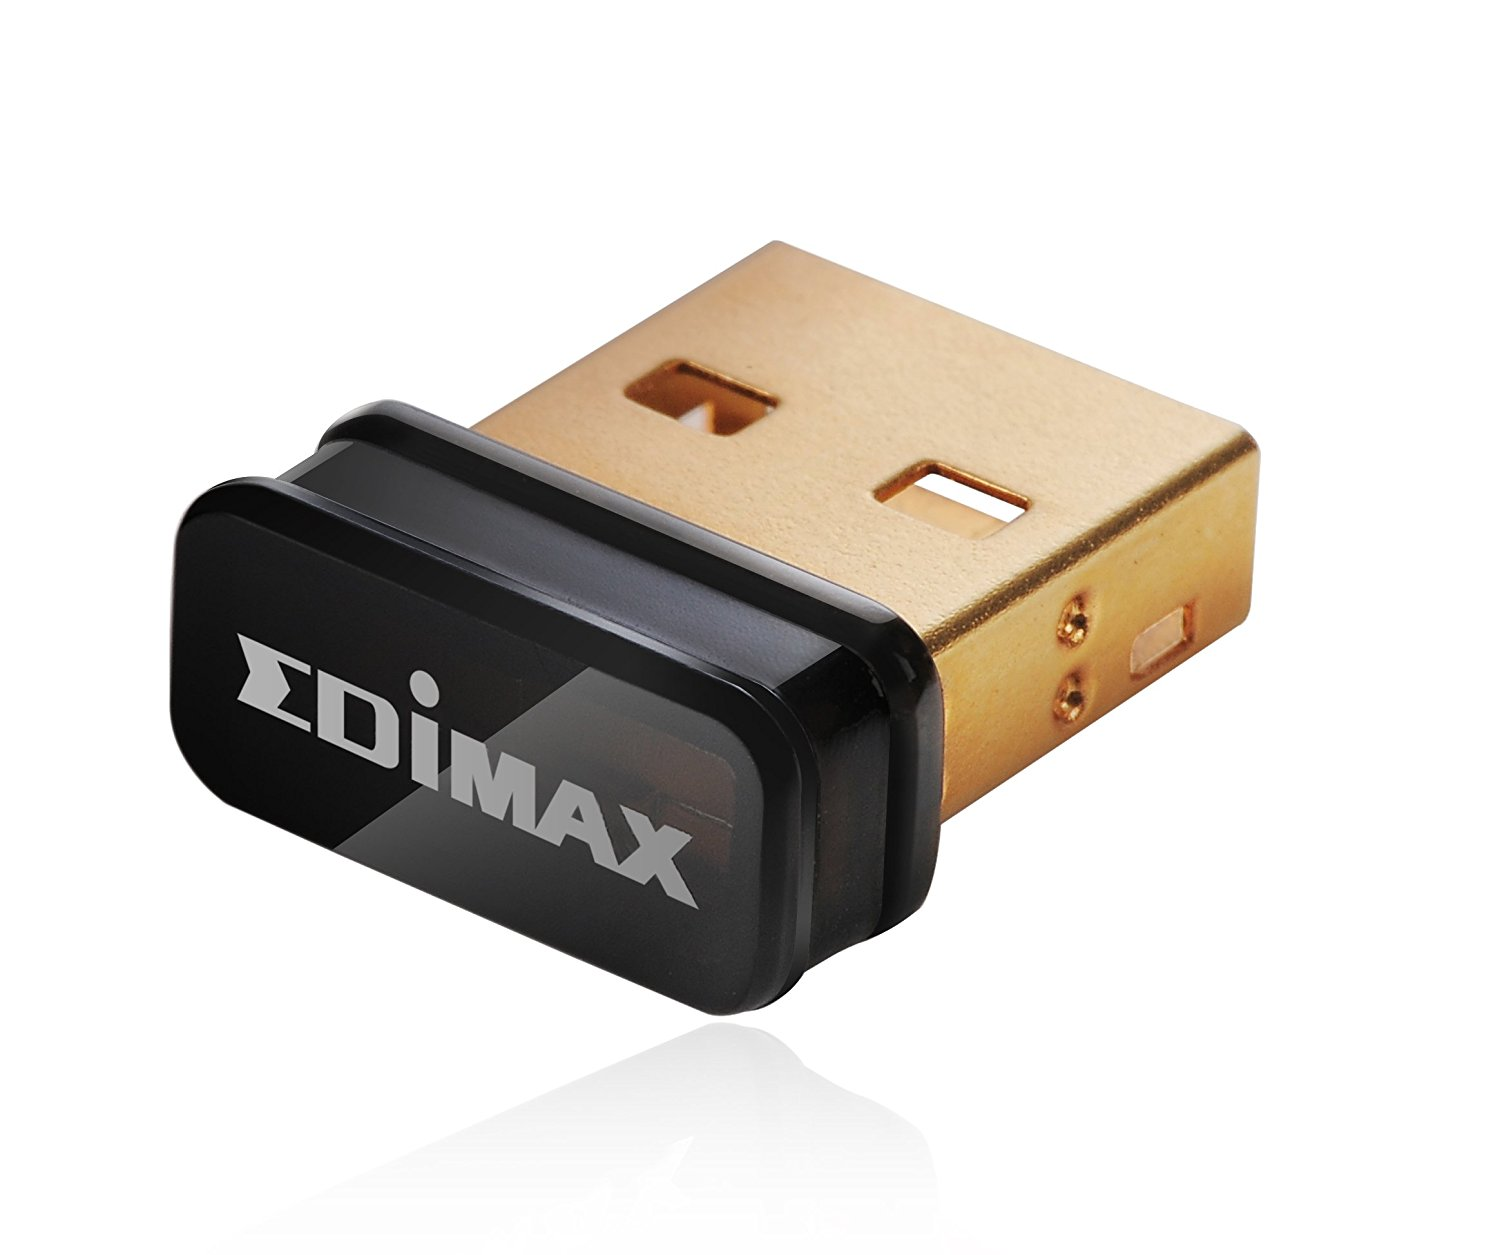
\includegraphics[width = 0.4\textwidth]{edimax}
\caption{Edimax EW-7811Un Wi-Fi adapter}
\label{fig::edimax}
\end{figure}

\section{Assembly}

In this section, the schematics of the assembled components has been analysed and given in figure \ref{fig::schematics}.

\begin{figure}[h] 
\centering
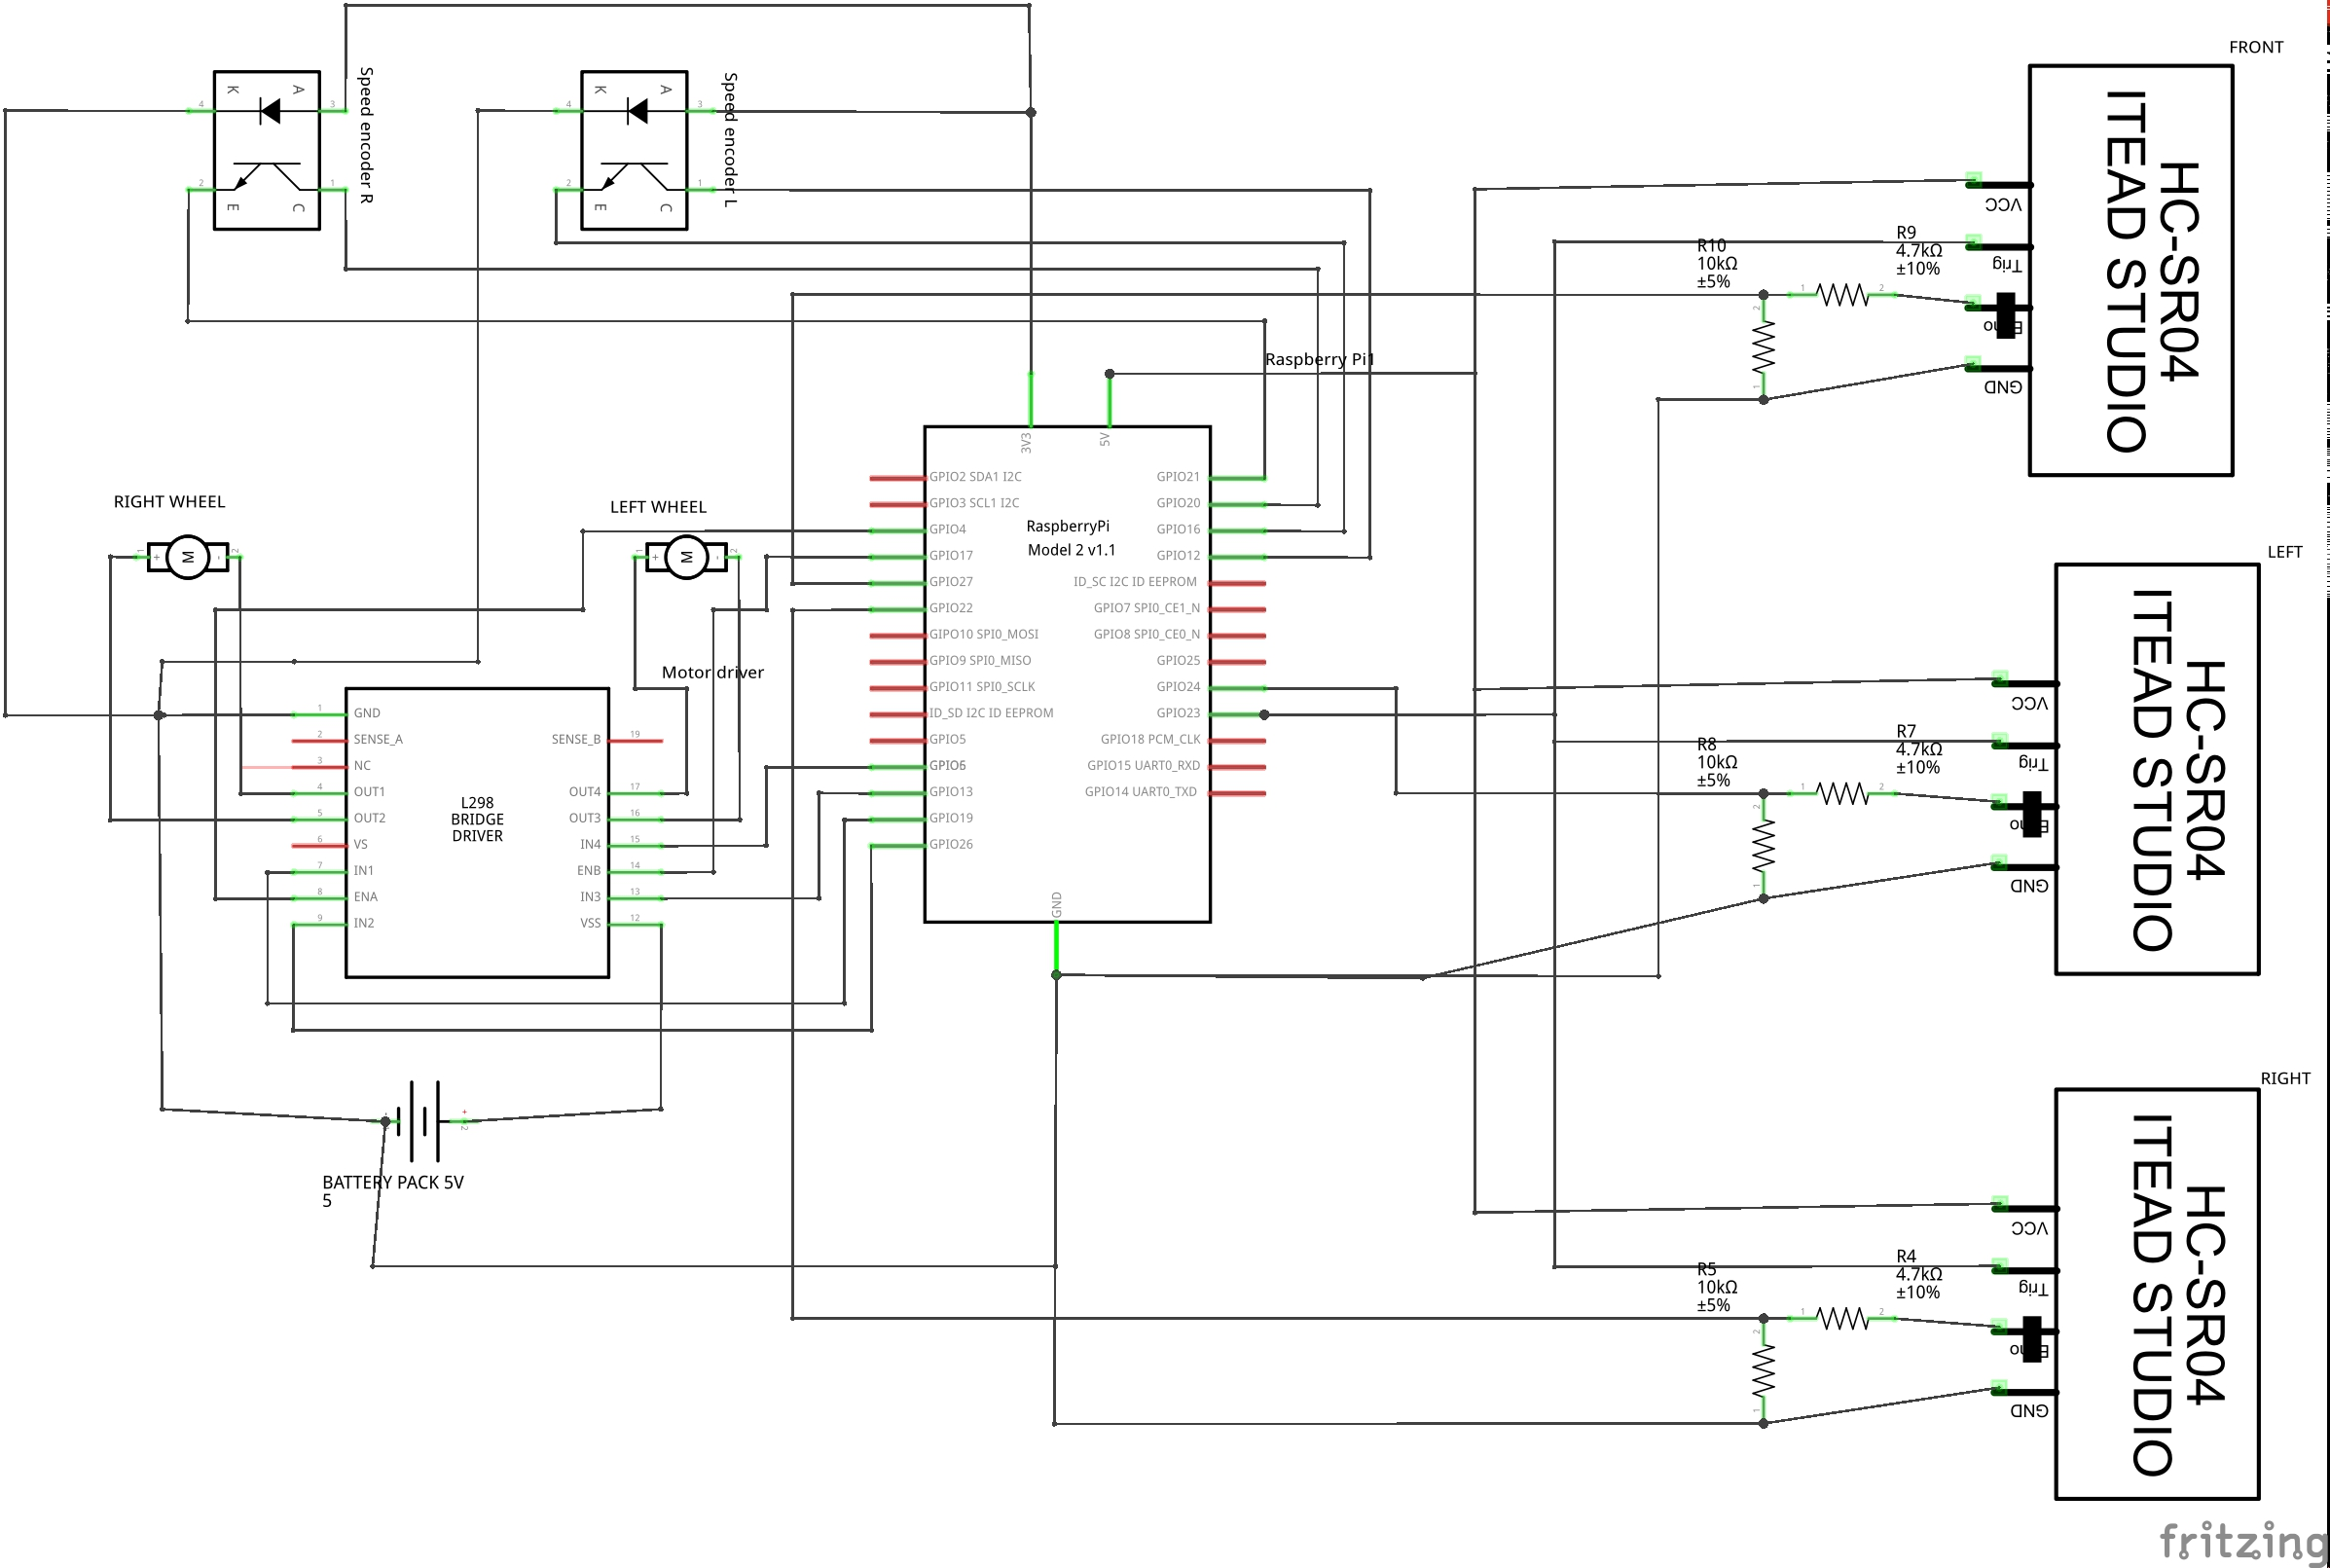
\includegraphics[width = 1\textwidth]{P51_schem}
\caption{Schematics of the device}
\label{fig::schematics}
\end{figure}

In the middle section of the schematics, the Raspberry Pi is present. Unfortunately, the software used to make this schematic did not have the Raspberry Pi Zero layout, so the model 2 was used instead. Regarding the project there is not a big difference, as the pins are the same as Zero.

On the right side of the system three ultrasonic sensors could be seen, connected to the Raspberry Pi. The Vcc and GND pins are all connected to the Raspberry, allowing the sensors to draw power from the microcontroller itself. The trigger pins are all connected to the same Raspberry pin, meaning that when one of the sensors is triggered all of them will emit sonic impulse.
The triggers are all on the same pin to not limit the number of available pins on the Raspberry. However there is not a significant difference,as the echo pins of each of the sensors go into separate ports on the Raspberry and each of them has a voltage divider connected to the GND.

The driver is present in the bottom left of the schematics, alongside a battery pack connected to the driver and providing power to both motors. It is connected to the Raspberry by six pins, four responsible for the direction of the motors(2 for each motor) and 2 enable pins, used for controlling the speed of the motor by PWM.

\newpage
The motors are connected directly to the driver, by two wires.
The two encoders, responsible for monitoring the speed of the wheels, are present in the top left of the schematics
An external power source was used for the Raspberry Pi, which is not present in this schematics.



\chapter{Modeling} \label{ch:modeling}

This chapter is concerned with the mathematical model of the wheeled robotic vehicle and will serve as a pre-requisite for the later implemented feedback control algorithm. 
The dynamics part, describing the motor model, will be used in the cruise control derivation. Subsequently the kinematics model, which treats the robot as a point entity, will be used in the estimation for position control.

\section{Differential Drive} \label{kin_model} 

Differential drive steering, a popular choice in mobile robots, is a design where two wheels on a same axle are controlled independently. It may or may not include a castor wheel, however this paper addresses the latter. Depending on the relative rotation of each wheel, the robot could be steered in a desired manner. For the sake of clarity, several basic cases of interest are presented along with the equations describing the linear and angular velocity of the vehicle. 

\begin{align}
v = \frac{Rw_r + Rw_l}{2} \label{eq1} \\
W = \frac{Rw_r - Rw_l}{l} \label{eq2} 
\end{align}

Equation \ref{eq1} describes the linear speed of the robotic vehicle, with respect to the angular speeds of each wheels (\textbf{$w_r$}) and (\textbf{$w_l$}) and the wheel radius (\textbf{R}), while \ref{eq2} describes the angular speed of the robot, with \textbf{l} being the axle length between the wheels. 
The equation could be rewritten in matrix form as:

\begin{equation}  	\label{eq3} 
\begin{pmatrix}
	v \\
	\omega	
\end{pmatrix} 
=
\begin{pmatrix} 
	\frac{R}{2} & \frac{R}{2} \\
	\frac{R}{l} & \frac{-R}{l} 
\end{pmatrix}
\begin{pmatrix}
	\omega_r \\
	\omega_l
\end{pmatrix}  	
\end{equation}

Analysis of the above equation leads to the consideration of three cases where certain behaviour is to be expected.

\begin{itemize} \label{list_v}

\item $\boldsymbol{v_r = v_l}$ \\ In this case scenario, both wheels have the same speed. The robot's speed from equation \ref{eq13} is simply equal to the individual speed of each of wheel. On the other hand, the angular speed from equation \ref{eq14} becomes 0, and the turning radius infinite. The robot is expected to perform straight linear motion.

\item $\boldsymbol{v_r = 0}$ or $\boldsymbol{v_l = 0}$ \\ In this case scenario, the turning radius becomes $\frac{l}{2}$. The robot is expected to perform rotation either about the right or the left wheel, with the center of rotation being the zero velocity wheel. 

\item $\boldsymbol{v_l = -v_r}$ \\ In this case scenario, the turning radius and the linear speed become 0, while the angular speed is doubled. The robot is expected to perform rotation about it's midpoint, or simply put in-place rotation.

\end{itemize}

\subsection{Non-holonomic constraints} 

A robot, using the differential drive steering design, has restricted local movements, while having no restrictions in global motion. \todo{Reference} That is similar to the restrictions on a car, where it is not possible to slide into a parallel position with respect to the current one. Nevertheless, the vehicle can still manoeuvre into the desired position, similar to parallel parking. 

If we consider \todo{insert vehicle figure} we can define the non-holonomic constraints of a differential drive vehicle as: 

\begin{equation} \label{eq4}
\dot{x}sin(\theta) - \dot{y}cos(\theta) = 0
\end{equation}

As observed from equation \ref{eq4} and shown by figure \ref{fig::xy_orient}, the robot can not have speed perpendicular to the sagittal axis. The equation can be further rewritten as:

\begin{equation} \label{eq5} 
\tan{\theta} = \frac{\dot{y}}{\dot{x}} = \frac{dy}{dx}
\end{equation} 
\\

\begin{figure}[h]
\centering
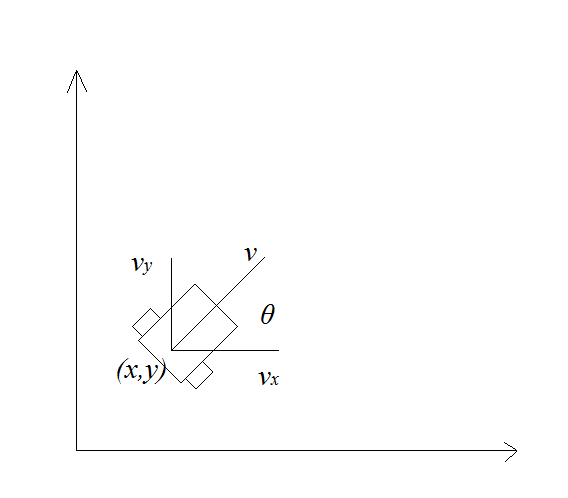
\includegraphics[width=0.5\textwidth]{Orientation_xy}
\caption{WMR orientation}
\label{fig::xy_orient}
\end{figure}

\section{Kinematics} \label{kinematics}

The kinematic model, similar to most rigid vehicles travelling on a two-dimensional plane, is of three degrees of freedom. From figure \ref{fig::xy_orient}, we can identify \textbf{x} and \textbf{y} as the coordinates for the center of mass of the robot and \textbf{$\theta$} as the angle with respect to the x axis. From the constraints of the vehicle, the equations concerning the kinematic model are derived as:

\begin{align}
\dot{x} = vcos(\theta) \nonumber \\
\dot{y} = vsin(\theta) \label{eq6} \\
\dot{\theta} = \omega  \nonumber 
\end{align}

Where \textbf{v} is the linear and \textbf{$\omega$} is the angular speed of the vehicle.
The equations could further be represented in matrix form.

\begin{equation} \label{eq7} 
\begin{pmatrix}
	\dot{x} \\
	\dot{y} \\
	\dot{\theta} \\ 
\end{pmatrix} 
=
\begin{pmatrix} 
	\cos{\theta} & 0 \\
	\sin{\theta} & 0 \\
	0     		 & 1  
\end{pmatrix}
\begin{pmatrix}
	v \\
	\omega
\end{pmatrix}  	
\end{equation}


%The relation between the linear speed and the angular speed of the robot is similar to equation \ref{eq12}.

%\begin{equation} \label{eq15} 
%v = WD
%\end{equation}

%Where D is the turning radius, from the midpoint of the wheels to the ICC. Solving for the turning radius, yields:

%\begin{align}
%D = \frac{v}{W} \label{eq16} \\
%= \frac{l}{2}\frac{v_r + v_l}{v_r - v_l} \nonumber
%\end{align}

\section{Dynamics} \label{dc_math}

%\begin{figure}[h] %change image
%\centering
%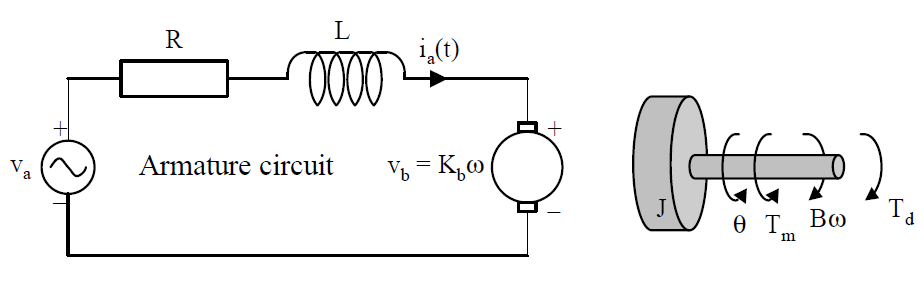
\includegraphics[width = 0.7\textwidth]{Motor_curcuit}
%\caption{Electrical circuit and free-body diagram of DC motor \cite{FBD}}
%\label{fig::motor_curcuit}
%\end{figure} 

In this section the equations used in the dynamics model of the motor are derived and described.

A DC motor produces mechanical torque applied to the shaft($\boldsymbol{T_e}$) linearly proportional to the armature current, the magnetic field and a torque constant($\boldsymbol{K_t}$). Assuming constant magnetic field, the produced torque is proportional to the torque constant($\boldsymbol{K_t}$) and the armature current(\textbf{I}).( Equation \ref{eq1})Furthermore, the back Emf (electromotive force)($E_b$) is equal to the angular velocity($\omega$) of the shaft multiplied with the Back emf constant($K_b$).(Equation \ref{eq2}) \\

\begin{align}  
T_e = IK_t \label{eq8}\\
E_b = \omega K_b \label{eq9}
\end{align}

Because the two constants $K_t$ and $K_b$ are equal in SI units, in further equations and simulations they will be denoted only as a motor constant $K$.

%VERIFY AND MODIFY

%\begin{equation} \label{eq3}
%K_t = K_b = K
%\end{equation} 

Using Kirchhoff's voltage law, the equations modelling the electrical part of the DC motor are derived as:

\begin{equation} \label{eq10}
V = RI + L\frac{dI}{dt} + E_b
\end{equation} 

where (\textbf{V}) is the applied voltage, (\textbf{R}) the armature resistance,(\textbf{L}) the armature inductance, ($\boldsymbol{E_b}$) the Back EMF. \ref{eq4}
Substitution ($\boldsymbol{E_b}$) with \ref{eq8} yields:

\begin{equation} \label{eq11}
V = RI + L\frac{dI}{dt} + K_b\omega
\end{equation}

The mechanical part of the DC motor(mechanical part of figure \ref{fig::motor_curcuit}) is described by Newton's second law for rotational motion as:

\begin{equation} \label{eq12}
J\dot{\omega} = K_tI - b\omega
\end{equation}

Where \textbf{J} is the load's inertia and \textbf{b} is the viscous friction in the motor's bearings.
Further substitution in equation \ref{eq4} with the derived back emf from \ref{eq2} results in:

Equations \ref{eq10} and \ref{eq11} are the equations describing the electrical and mechanical part of the motor.

Applying the Laplace transform to the equations \ref{eq10} and \ref{eq11}, we can relate the output angular velocity to the input voltage as described in the transfer function:

\begin{equation} \label{eq13}
\frac{\Omega(s)}{V(s)} = \frac{K_t}{(Js + b)(sL + R) + K_tK_b}
\end{equation}

The state space form representation of equations \ref{eq10} and \ref{eq11} is represented in the form $\dot{x} = Ax + Bu$ , where the state variables are the current (\textbf{I}) and the angular speed ($\boldsymbol{\omega}$)

\begin{equation} \label{eq14} 
\begin{pmatrix}
	\dot{I} \\
	\dot{\omega} \\
\end{pmatrix} 
=
\begin{pmatrix} 
	\frac{-b}{J}   & \frac{-K_t}{J} \\
	\frac{-K_b}{L} & \frac{-R}{L} \\ 
\end{pmatrix}
\begin{pmatrix}
	I \\
	\omega
\end{pmatrix}
+
\begin{pmatrix}
	\frac{1}{L} \\
	0
\end{pmatrix}
V	
\end{equation}


The Simulink block diagram describing the behaviour of the DC motor in continuous time is given in figure \ref{fig::motor_block}.

\begin{figure}[h]
\centering
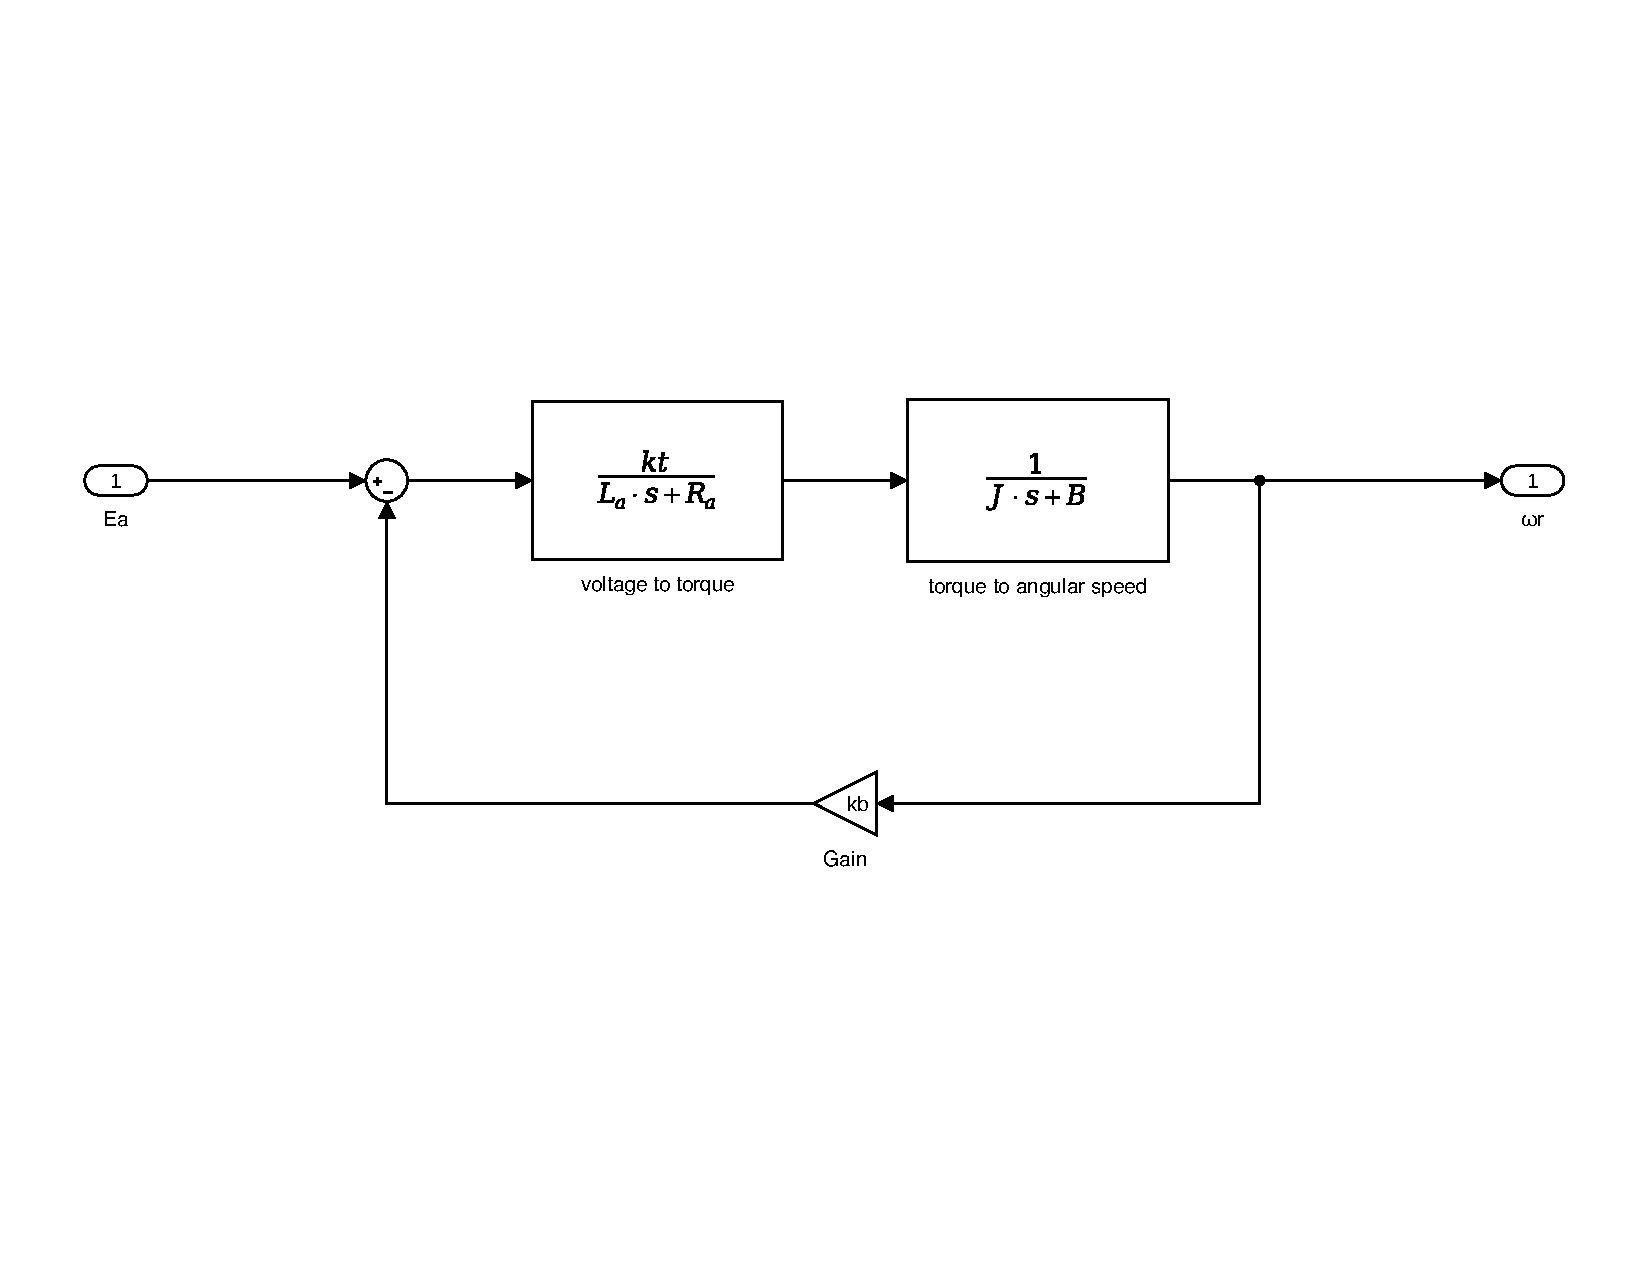
\includegraphics[width=0.5\textwidth]{dcmodel}
\caption{Motor block diagram}
\label{fig::motor_block}
\end{figure}

The motor model is a SISO system, where the input is Voltage and the output is angular velocity. Thus, classical control is sufficient to manipulate the behaviour of the system.  

\section{Complete Model} 

Combining the motor dynamics, the the robot kinematics yield the complete plant of the system.

\section{Dead reckoning} 

If we consider the robot's configuration \textbf{q}, previously described as (x,y,$\theta$), a way of measuring the above mentioned configuration is required in order to implement planning and feedback control. Incremental encoders are common in wheeled robots as they are able to measure the rotation of the wheels. However, they do not provide direct measurements of the position and orientation of the robot, thus dead reckoning (aka. odometric localization) is an affordable way to estimate the vehicle's configuration \textbf{q} by iterative integration of the kinematic model from \ref{kinematics}. The major drawback of the method is the proneness to error, that is if there exists a small error in any step of the localization it will influence the calculation of the subsequent positions, leading to potentially large deviation between the expected position and the localization results. From that we can conclude that dead reckoning is less precise in large areas due to systematic errors( eg. limited encoder resolution, unequal wheel diameters, etc.), and external factors not considered in the kinematics due to non-systematic errors( eg. wheel slippage on floors, inclined surfaces etc.) \todo{ref book Modelling.Planning and Control}

Assuming constant inputs $\boldsymbol{v_k}$ and $\boldsymbol{\omega_k}$ in the kinematic model \ref{kinematics} for discrete time [$t_k$,$t_{k+1}$] (zero-order hold), for the sampling step \textbf{k} =1,2,...,n, the differential drive robot will traverse along an arc with a circle radius \textbf{D} ($\frac{v_k}{\omega_k}$). Furthermore if the starting position ($x_k$,$y_k$,$\theta_k$), for \textbf{k} =1, and the velocities $\boldsymbol{v_k}$ and $\boldsymbol{\omega_k}$ are known, we can reconstruct the value of ($x_{k+1}$,$y_{k+1}$,$\theta_{k+1}$) by forward integration of the kinematic model at the sampling time $t_{k+1}$. Several methods for numerical integration could be used, among which are the Forward Euler method, Second-order Runge-Kutta method or exact integration. \todo{ref Robotics book}. Because of inadequate accuracy due to the constant orientation $\theta_k$ in the Euler method, in this paper we will consider the Runge-Kutta approximation method and exact integration as described in the book "Robotics: Modelling, Planning and Control" by Bruno Siciliano.

\begin{align}
x_{k+1} = x_k + T_s v_k cos(\theta_k + \frac{\omega_k T_s}{2}) \\
y_{k+1} = y_k + T_s v_k sin(\theta_k + \frac{\omega_k T_s}{2}) \label{eq15} \\
\theta_{k+1} = \theta_k + T_s\omega_k  \nonumber 
\end{align}

Equation \ref{eq15} refers to the second-order Runge-Kutta method, where $\boldsymbol{T_s}$ is the duration of the sampling period $T_s = t_{k+1} - t_k$. It is important to note that the approximations for $x_{k+1}$ and $y_{k+1}$ use the average value of the unicycle orientation in the sampling period, compared to the less accurate Euler method with constant orientation.

The exact reconstruction of ($x_{k+1}$,$y_{k+1}$,$\theta_{k+1}$), assuming constant velocity inputs in the sampling interval is given by \ref{}:\todo{reference to book} 

\begin{align}
x_{k+1} = x_k + \frac{v_k}{\omega_k}(sin(\theta_{k+1} - sin(\theta_k)\\
y_{k+1} = y_k + \frac{v_k}{\omega_k}(cos(\theta_{k+1} - cos(\theta_k) \label{eq16} \\
\theta_{k+1} = \theta_k + T_s\omega_k  \nonumber 
\end{align}

Note that the exact reconstruction is not defined for $w_k$ = 0 (motion in a line segment) thus, in implementation, a conditional statement has to handle the exception by using the Runge-Kutta method, which is still defined for $w_k$ = 0.

Nevertheless, in practice it is convenient to estimate the input velocities using the incremental encoders	and by calculating the relative displacement $\Delta s$ and orientation $\Delta\theta$  over the sampling period:

\begin{align}
v_k T_s = \Delta s \nonumber \\
\omega_k T_s = \Delta\theta \label{eq17} \\
\frac{v_k}{\omega_k} = \frac{\Delta s}{\Delta\theta} \nonumber
\end{align}

In the case of a differential drive robot with a castor wheel, from equation \ref{eq1} and \ref{eq2}, we can define $\Delta s$ and $\Delta\theta$ as :

\begin{align}
\Delta s 	 = \frac{r}{2}(\Delta s_r + \Delta s_l) \label{eq18} \\
\Delta\theta = \frac{r}{l}(\Delta s_r - \Delta s_l) \nonumber
\end{align}

Where $\Delta s_r$ and  $\Delta s_l$ are the rotation of the right and left wheel, respectively, measured by the incremental encoders during the sampling period. 


\section{System Parameters} \label{parameter}

In this section the parameters used in the mathematical model of the robot are given. They were acquired by measurements and experiments on the physical system, prior to implementation.

\begin{table}[h]
\centering
\begin{tabular}{cccll}
\hline
Parameter                   & Description                               & Nominal Value                                 &  &  \\ \hline
\multicolumn{1}{|c|}{K}     & \multicolumn{1}{c|}{Motor constant}       & \multicolumn{1}{c|}{0.1838 V/(rad/s)  Nm/amp} &  &  \\ \cline{1-3}
\multicolumn{1}{|c|}{R}     & \multicolumn{1}{c|}{Armature resistance}  & \multicolumn{1}{c|}{11.5 $\Omega$}            &  &  \\ \cline{1-3}
\multicolumn{1}{|c|}{L}     & \multicolumn{1}{c|}{Armature inductance}  & \multicolumn{1}{c|}{0.1 H}                    &  &  \\ \cline{1-3}
\multicolumn{1}{|c|}{$b_r$} & \multicolumn{1}{c|}{Rotor damping}        & \multicolumn{1}{c|}{0.0221}                   &  &  \\ \cline{1-3}
\multicolumn{1}{|c|}{$J_w$} & \multicolumn{1}{c|}{Load inertia} & \multicolumn{1}{c|}{2.8033e-5 $KgM^2$}        &  &  \\ \cline{1-3}
\multicolumn{1}{|c|}{n}     & \multicolumn{1}{c|}{Gear ratio}           & \multicolumn{1}{c|}{1:48}                     &  &  \\ \cline{1-3}
\multicolumn{1}{l}{}        & \multicolumn{1}{l}{}                      & \multicolumn{1}{l}{}                          &  &  \\ \hline
\end{tabular}
\caption{System parameters}
\label{sys_par}
\end{table}

\todo{include all parameters} 

 
\chapter{Development}\label{ch:development}

\paragraph{Hardware testing} 

\section{Ultrasonic sensors} \label{us_test}

The first part of the hardware outline was testing of the ultrasonic sensors.
For each of the sensors a voltage divider was build as seen on figure /ref{voltage1}.

\begin{figure}[h]
\centering
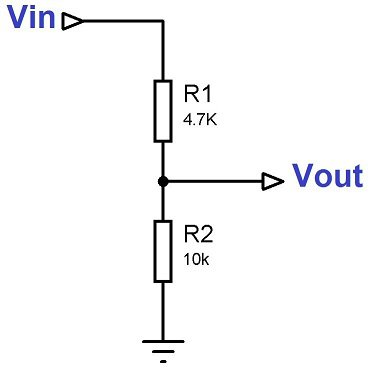
\includegraphics[width = 0.5\textwidth]{voltage1}
\caption{Voltage divider}
\label{fig::voltage1}
\end{figure}

The values of the resistors are calculated by the following equation:
\begin{equation} \label{voltagedivider} 
{V}_{out}={V}_{in}*{R}_{2}/({R}_{1}+{R}_{2})
\end{equation}

All sensors were tested out separately by connecting them individually to the Raspberry pi and running the test code below

\begin{lstlisting}
import RPi.GPIO as GPIO
import time
GPIO.setmode(GPIO.BCM)

TRIG = 23
ECHO = 24

print "Measuring distance"

GPIO.setup(TRIG, GPIO.OUT)
GPIO.setup(ECHO, GPIO.IN)

while True:
	GPIO.output(TRIG, False)
	print "Waiting for the sensor"
	time.sleep(2)

	GPIO.output(TRIG, True)
	time.sleep(0.00001)
	GPIO.output(TRIG, False)

	while GPIO.input(ECHO)==0:
		pulse_start = time.time()

	while GPIO.input(ECHO)==1:
		pulse_end= time.time()

	pulse_duration = pulse_end - pulse_start

	distance = pulse_duration * 17150
	distance = round(distance, 2)

	print "Distance:%d",distance

\end{lstlisting}

Each of the sensors worked as expected while connected separately, thus the logical progression was to test them out all at the same time.
While taking the readings, it was noticeable that some of the values where random or distorted due to noise and could not be used for accurate measurement. Therefore, some filtering had to be included in order to scale the values to an acceptable limit. A moving average filter was used for the previously mentioned task by taking three reading at a time and calculating the average of the values. 

\begin{lstlisting}
def readsensor(PIN):
	for x in range(0, 2):
		read_time_start1 = time.time()
		GPIO.output(TRIG, True)
		time.sleep(pulse)
		GPIO.output(TRIG, False)

		while GPIO.input(PIN)==0:
			pulse_start = time.time()

		while GPIO.input(PIN)==1:
			pulse_end= time.time()

		pulse_duration[x] = pulse_end - pulse_start
		time.sleep(0.05-(time.time()-read_time_start1))

	distance = sum(pulse_duration)/measurment_count* SPEED_OF_SOUND
	distance = round(distance, 2)
	print distance
while True:
	readsensor(ECHOF)
	readsensor(ECHOR)
	readsensor(ECHOL)
	
\end{lstlisting}

From the code above, the application of the moving average filter could be seen. Importantly there was a noticeable improvement of the readings, which became much more precise and consistent.
Furthermore, it can be seen that every reading takes less than 0.05 seconds. This is useful in making every cycle evenly long and predictable, when it comes to the total time that the program is required to run the full cycle. Therefore the time for the full sensor reading loop becomes $3\times0.05s=0,15s$.

\section{DC motors}
To make sure the purchased DC motors were operational an initial testing was performed by driving each of them in forward and in backward gear through the used driver. This can be seen in script below.

\begin{lstlisting}
GPIO.setmode(GPIO.BCM)
GPIO.setup(StepPinForward, GPIO.OUT)
GPIO.setup(StepPinBackward, GPIO.OUT)

def forward(x):
    GPIO.output(StepPinForward, GPIO.HIGH)
    print "forwarding running  motor "
    time.sleep(x)
    GPIO.output(StepPinForward, GPIO.LOW)

def reverse(x):
    GPIO.output(StepPinBackward, GPIO.HIGH)
    print "backward running motor"
    time.sleep(x)
    GPIO.output(StepPinBackward, GPIO.LOW)

print "forward motor "
forward(5)
print "reverse motor"
reverse(5)

print "Stopping motor"
GPIO.cleanup()

\end{lstlisting}

As it can be seen from the code, one of the motors was initially driven forward for 5 seconds and subsequently backwards for 5 seconds. To apply the test for the second motor simply the pin numbers(StepPinForward and StepPinBackward) were changed.

Furthermore, Pulse Width Modulation (PWM) was utilized in order to regulate the separate speeds of the motors, as it was an initial condition to implement cruise control.
in the final software what is ran on the device we have changed the forward() and reverse() so that we can change the speed of the motors at our desire.

\begin{lstlisting}
 def forward(forwardtime,SPEED):
	print "REVERSE"
	GPIO.output(StepPinBackward1, GPIO.HIGH)
	GPIO.output(StepPinBackward2, GPIO.HIGH)
	PWML.start(SPEED)
	PWMR.start(SPEED)
	time.sleep(forwardtime)
	GPIO.output(StepPinBackward1, GPIO.LOW)
	GPIO.output(StepPinBackward2, GPIO.LOW)
\end{lstlisting}

As you can see from the code above we use the drivers PWM input to change the speed of the vehicle.

\section{Raspberry Pi configuration and software}

In this section, a description of the steps taken to configure the Raspberry Pi, was made.

\subsection{Raspberry setup}

Initially, after obtaining the Raspberry Pi Zero, an installation of the Raspbian OS was performed.
Subsequently, all GPIO pins were enabled, followed by configuration of the Secure Shell (SSH) protocol in order to perform remote logins to the microcontroller. Furthermore, as mentioned in the Hardware chapter, due to it's size, the Raspberry Zero has only one USB port, resulting in a space limitation. Thus, the logical choice was to connect the Wi-Fi adapter to that USB port, and configure the microcontroller remotely, through the SSH. 
Additionally, extra tools such as Tmux Multitab and Nano Text Editor were used to clarify the programming sessions.

\subsection{Software}

The software constituting the robot's behaviour is self-made with the addition of several external libraries 

\begin{lstlisting}
import sys
import time
import RPi.GPIO as GPIO
\end{lstlisting}

To be precise, only three external libraries were used at the time of the development of this paper. Nevertheless, as the system is still in active development the list may expand after the submission of the documentation.

\begin{itemize}

\item \textbf{Sys module} \\ This module provides a number of functions and variables that can be used to manipulate different parts of the Python runtime environment. \cite{sys_module}

\item \textbf{Time module} \\ This module provides a number of functions to deal with dates and the time within a day. It is a thin layer on top of the C runtime library.
A given date and time can either be represented as a floating point value (the number of seconds since a reference date, usually January 1st, 1970), or as a time tuple. \cite{time_module}

\item \textbf{RPi.GPIO module} \\ This module is for functions that are connected to the GPIO pins.
\end{itemize}

The overall setup of the pins and the variables, with the different values used in the code, is present in the snippet below.

\begin{lstlisting}
#PIN numbers
LetfPWM=16
RightPWM=20
StepPinForward1=26
StepPinBackward1=19
StepPinForward2=13
StepPinBackward2=6
ECHOF=4
ECHOL=27
ECHOR=22
TRIG=17

#Values for reading the sesnsors
SPEED_OF_SOUND = 17150
measurment_count = 3
pulse = 0.00001	
pulse_duration = [0,0,0]
sensorF_data=0
sensorR_data=0
sensorL_data=0

#navigation variables
reversetime=0
turningtime = 1
MAXSPEED = 1
MEDSPEED = 0.6
MINSPEED = 0.1

#GPIO setup for each pin 
GPIO.setmode(GPIO.BCM)
GPIO.setup(StepPinForward1, GPIO.OUT)
GPIO.setup(StepPinBackward1, GPIO.OUT)
GPIO.setup(StepPinForward2, GPIO.OUT)
GPIO.setup(StepPinBackward2, GPIO.OUT)
GPIO.setup(ECHOF, GPIO.IN)
GPIO.setup(ECHOL, GPIO.IN)
GPIO.setup(ECHOR, GPIO.IN)
GPIO.setup(TRIG, GPIO.OUT)
GPIO.setup(LetfPWM, GPIO.OUT)
GPIO.setup(RightPWM, GPIO.OUT)

#PWM channels and frequency
PWML=GPIO.PWM(16, 0.5)
PWMR=GPIO.PWM(20, 0.5)
\end{lstlisting}

\subsection{Ultrasonic sensor reading}


As previously mentioned, the ultrasonic sensors are the proposed way of implementing collision detection. The desired function is for them to measure the distance from the robot to the closest present obstacle, and return the data for further usage in the code.
In subsection \ref{us_test}, it was mentioned of the potential problems with noise and the proposed filtering method, using the average of every three reading. 
Below is a section of the code, with the function for data acquisition after filtering the readings.

\begin{lstlisting}
 def readsensor(PIN):
	for x in range(0, 2):
		read_time_start1 = time.time()
		GPIO.output(TRIG, True)
		time.sleep(pulse)
		GPIO.output(TRIG, False)

		while GPIO.input(PIN)==0:
			pulse_start = time.time()

		while GPIO.input(PIN)==1:
			pulse_end= time.time()

		pulse_duration[x] = pulse_end - pulse_start
		time.sleep(0.05-(time.time()-read_time_start1))

	distance = sum(pulse_duration)/measurment_count* SPEED_OF_SOUND
	distance = round(distance, 2)
	print distance
	if PIN == ECHOF:
		sensorF_data=distance

	if PIN == ECHOR:
		sensorR_data=distance

	if PIN==ECHOL:
		sensorL_data=distance
\end{lstlisting}

The data reading is straightforward. The \textbf{TRIG} pin emits an ultrasonic impulse from a each of the sensors in addition to a digital timestamp that records the exact time of the event. When the impulse reaches back the sensor, a second timestamp is recorded. The logic behind it is that every loop should take equal amount of time for execution. 
The first timestamp in the beginning of the loop is initialized with \textbf{$read_time_start1 = time.time().$} and calculated afterwards in \textbf{$time.sleep(0.05-(time.time()-read_time_start1))$}. The expected cycle length is 0.05 second and is done to ensure that reading are acquired in the sensing range 0.02m to 4m.
The set time of 0.05 second is used, as it would give the range, limited by time.

\begin{equation}
330(m/s)*0.05s=16.5
\end{equation}

And since the impulse is going to the object in range and returning to the sensor, a division by 2 with give the max range for the time limitation 

\begin{equation}
16.5/2=8.25m
\end{equation}

The result is almost double the sensing range supported by the hardware. 

Furthermore, from the line: for x in range(0, 2): the reading of the sensor is done 3 times in a row, thus the implementation of the moving average filter.

The last lines of code ensure that when data reading is initiated, it would pass the value to only one of the readings, avoiding data collision.

\begin{lstlisting}
	if PIN == ECHOF:
		sensorF_data=distance

	if PIN == ECHOR:
		sensorR_data=distance

	if PIN==ECHOL:
		sensorL_data=distance

\end{lstlisting}

\subsection{Movements}

The expected movements of a differential drive robot was covered in section \ref{kin_analysis}. In this subsection, a description is conducted on the pre made functions governing the behaviour of the physical system. It is important to mention  
  
At the completion of this chapter, five different functions concerned with the movements, have been used.

The most basic function is the \textbf{stop()}, which as it's name suggests, halts the motion of the device

\begin{lstlisting}
def stop():
	GPIO.output(StepPinForward1, GPIO.LOW)
	GPIO.output(StepPinForward2, GPIO.LOW)
	GPIO.output(StepPinBackward1, GPIO.LOW)
	GPIO.output(StepPinBackward2, GPIO.LOW)
\end{lstlisting}

All the movement enabling pins will be set to low, which prompts the device to halt any ongoing movements. 

The second function is the forward motion.

\begin{lstlisting}
 def forward(SPEED):
	print "FORWARD"
	GPIO.output(StepPinForward1, GPIO.HIGH)
	GPIO.output(StepPinForward2, GPIO.HIGH)
	PWML.start(SPEED)
	PWMR.start(SPEED)
\end{lstlisting}

From the code snippet, it can be seen that when the forward function is executed, both of the motors start moving in the same direction and the speed is determined by the variable SPEED. It is important to mention that small fluctuations in the speed of each wheel will cause curved motion instead of the desired forward linear motion, as discussed in section \ref{kin_analysis}. Thus appropriate control needs to be applied in order to maintain equal speed in both wheels. 

How the speed is determined will be further discussed in subsection \ref{main_loop}: main loop.

The third function is the reverse, or what is essentially the same as the forward function only that the triggered pins are the backward ones. As in the forward movements, appropriate control is needed to maintain backward linear motion.

\begin{lstlisting}
 def reverse(SPEED):
	print "REVERSE"
	GPIO.output(StepPinBackward1, GPIO.HIGH)
	GPIO.output(StepPinBackward2, GPIO.HIGH)
	PWML.start(SPEED)
	PWMR.start(SPEED)
\end{lstlisting}

The two movements: forward and backward are the essential functions for the robot's linear motion.

Next we have the turning functions left() and right().
It was decided that the turning functions should be made that the vehicle takes the least amount of space to turn.
As it was explained in section \ref{kin_model},in a differential drive if the velocities of each wheel are the same but in a different direction, the robot will rotate around its middle point of the wheel axis, which essentially becomes the turning radius.

Below are the two functions needed for turning.

\begin{lstlisting}
 def right(turningtime,SPEED):
	print "RIGHT"
	GPIO.output(StepPinBackward1, GPIO.HIGH)
	GPIO.output(StepPinForward2, GPIO.HIGH)
	PWML.start(SPEED)
	PWMR.start(SPEED)
	sleep(turningtime)
	GPIO.output(StepPinBackward1, GPIO.LOW)
	GPIO.output(StepPinForward2, GPIO.LOW)

def left(turningtime,SPEED):
	print "LEFT"
	GPIO.output(StepPinForward1, GPIO.HIGH)
	GPIO.output(StepPinBackward2, GPIO.HIGH)
	PWML.start(SPEED)
	PWMR.start(SPEED)
	sleep(turningtime)
	GPIO.output(StepPinForward1, GPIO.LOW)
	GPIO.output(StepPinBackward2, GPIO.LOW)
\end{lstlisting}

As we can see both turns, right and left, are made with predetermined factor \textbf{turningtime}.
This will ensure that the vehicle will not over or under turn.
And since a decision was made to mount 3 ultrasonic sensors, the turning ratio on 90 degrees was found adequate.
Alteration of the turningtime will allow the device to turn to any desired amount of degrees, however a requirement of more than three ultrasonic sensors and specific positioning might be necessary.

\subsection{Main loop} \label{main_loop}

In this subsection the main loop, initiated when the device starts, is analysed.

\begin{lstlisting}
while True:
	readsensor(ECHOF)

	if sensorF_data>200:
		forward(MAXSPEED)
		
	if 200>sensorF_data>100:
		forward(MEDSPEED)

	if 100>sensorF_data>20:
		forward(MINSPEED)

	if 20>sensorF_data:
		stop()
		readsensor(ECHOR)
		readsensor(ECHOL)

		while sensorR_data<15 and sensorL_data<15:	
			reverse(MINSPEED)
			readsensor(ECHOR)
			readsensor(ECHOL)
			
		if sensorR_data>sensorL_data== True:
			right(1,MINSPEED)
			break
			
		if sensorL_data>sensorR_data==True:
			left(1,MINSPEED)
			break
\end{lstlisting}

The loop is initiated with reading of the front sensor \textbf{readsensor(ECHOF)}. Any further action is determined, based on the reading taken from it. If the distance to the closest object is over 2m the vehicle will start moving in a forward direction with full speed. When the distance drops down between 200 cm and 100 cm, the vehicle speed will be reduced to medium speed in order to prepare for a potential turning. Minimal speed is initiated when the distance from the front sensor drops down between 100cm and 20cm, allowing the robot to perform an instant stop. 
When the distance to the closet object falls under 20 cm,the vehicle will stop and will decide how to proceed based on 3 possible cases. The ultrasonic sensors on the left and right will estimate the distance to the closest object on both sides.

\begin{itemize}

\item Case 1 \\ If both sides fall under 15 cm of the closest object, the robot will perform reverse motion and constantly recheck if space becomes available on either side. Once that is true, the robot will perform appropriate turn. 
\item Case 2 \\ If one or both of the side sensors register distance to the closest object more than 15 cm, it will turn in the direction of the larger available space.
\item Case 3 \\ If the robot performs a turn with a minimal acceptable distance reading, it will re-evaluate the possible turning options.

\end{itemize}

After the turning phase the loop will go back to the beginning and start all over again.

The loop is made as simple as possible to avoid any complications while running the code.

\section{N.B.}

Unfortunately, due to shipping delays, the completion of this part was done without the acquisition of the optical encoders, necessary to implement the crucial wheel speed control. Obstacle avoidance was performed, relying on the similarity of the motors, and was sufficient to successfully test the above mentioned code. After the arrival of the encoders (which is after the completion of this paper),a thorough update would be performed on this chapter and presented in order at the examination date. 
\chapter{Conclusion}\label{ch:conclusion}
In case you have questions, comments, suggestions or have found a bug, please do not hesitate to contact me. You can find my contact details below.
  \begin{center}
    Jesper Kjær Nielsen\\
    \href{mailto: jkn@es.aau.dk}{jkn@es.aau.dk}\\
    \href{http://kom.aau.dk/~jkn}{http://kom.aau.dk/\textasciitilde jkn}\\
    Fredrik Bajers Vej 7\\
    9220 Aalborg Ø
  \end{center}

\label{bib:mybiblio}
\appendix
\chapter{Driver Chip}\label{ch:appAlabel}

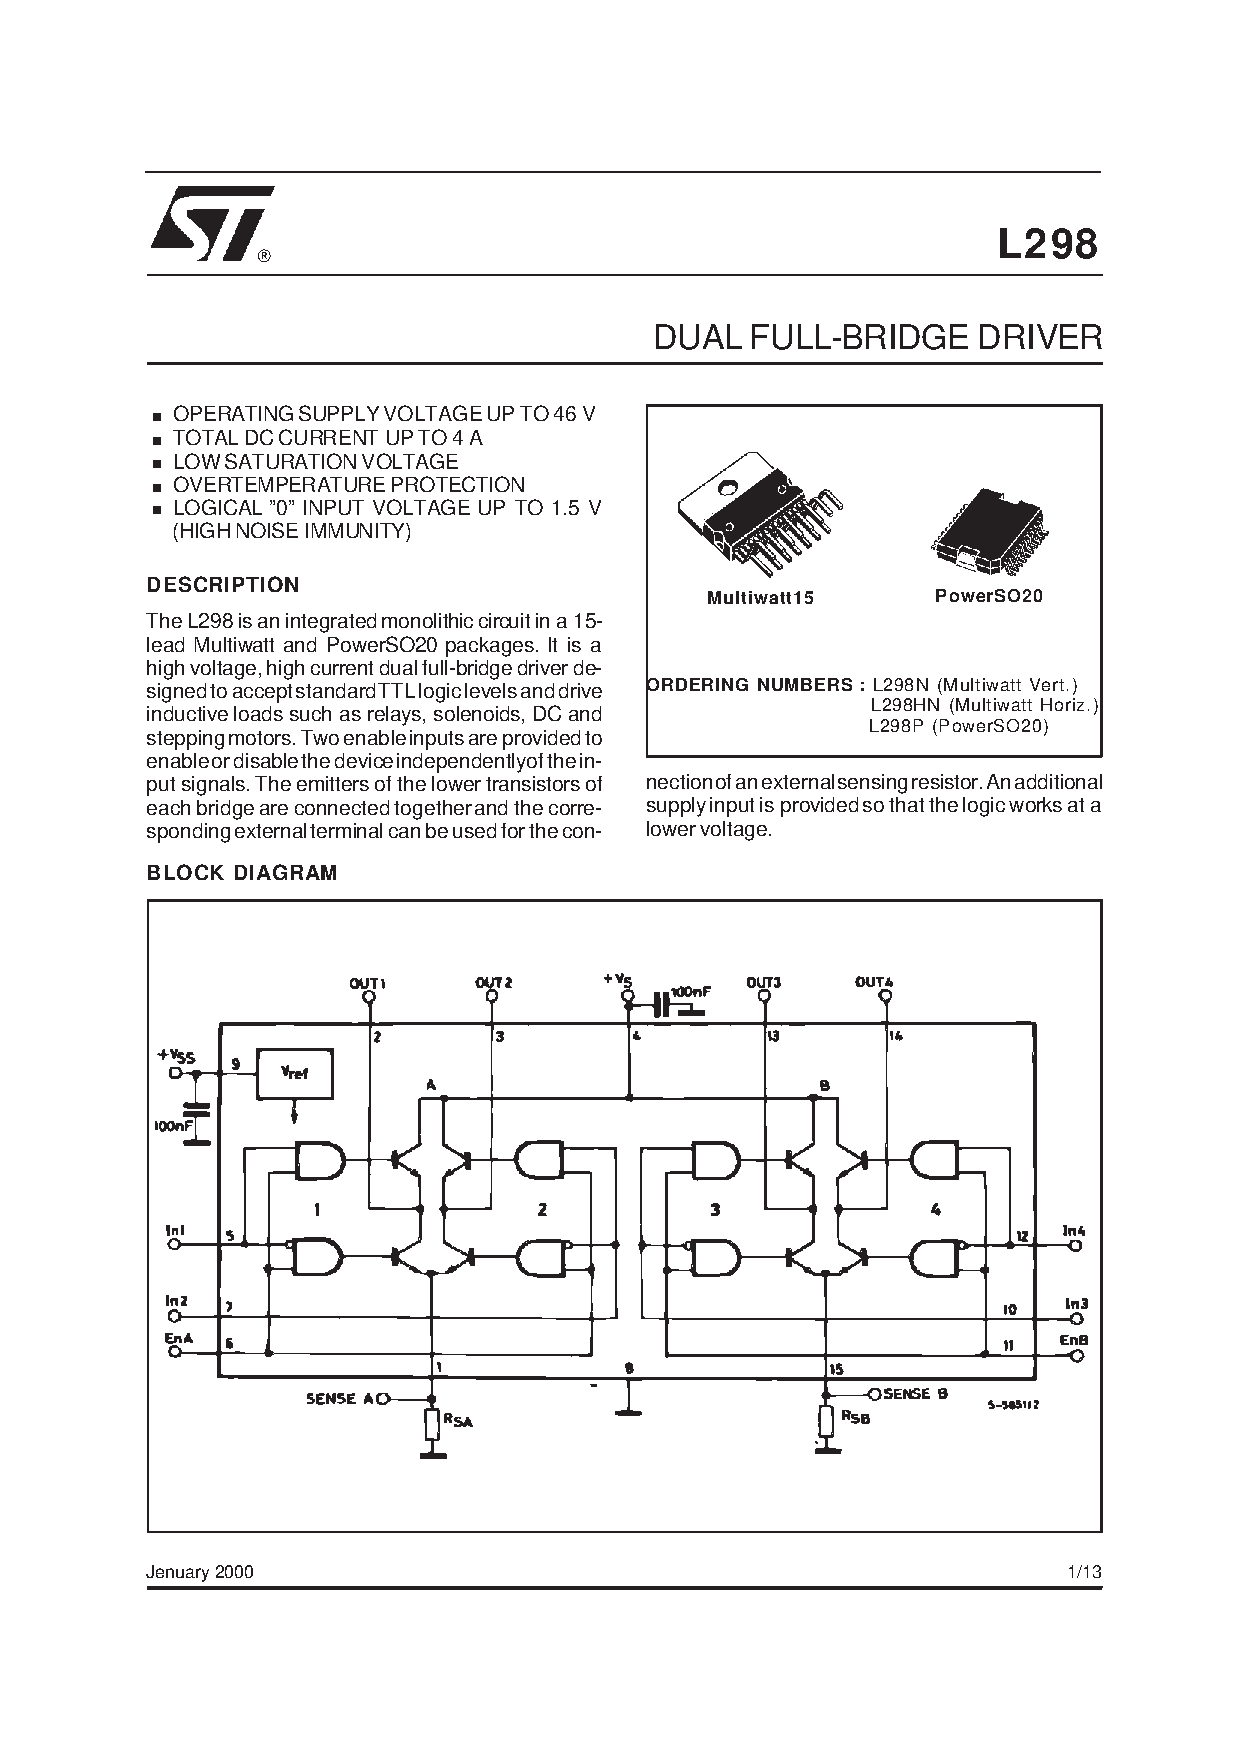
\includepdf[
pages=-,
width=1.6\textwidth,
height=1\textheight,
angle=0,
pagecommand =\section*{Driver Chip}]{datasheets/driverchip.pdf}


\chapter{Wi-Fi Adapter}\label{ch:appAlabel}

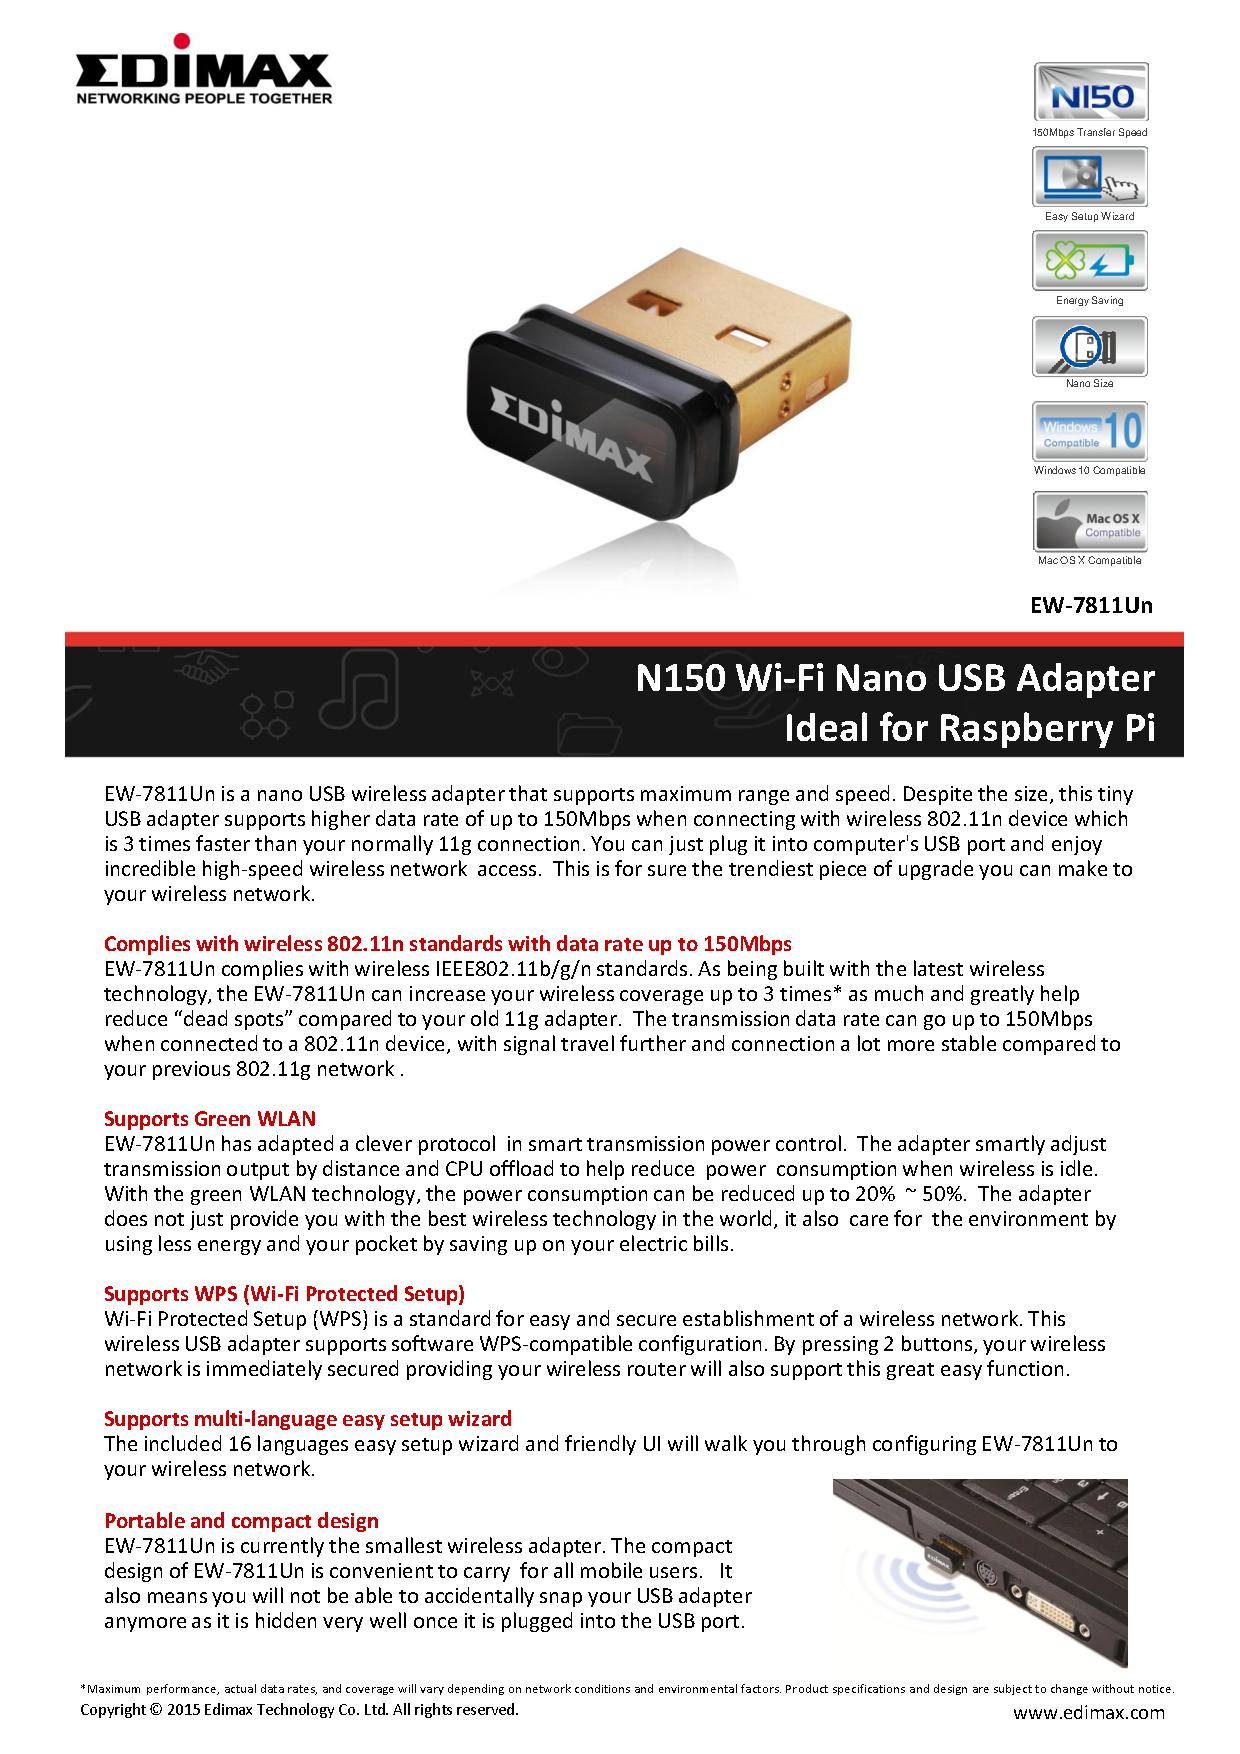
\includepdf[
pages=-,
width=1.6\textwidth,
height=1\textheight,
angle=0,
pagecommand =\section*{Wi-Fi Adapter}]{datasheets/EW-7811Un_Datasheet_English.pdf}


\chapter{Ultrasonic Sensor}\label{ch:appAlabel}

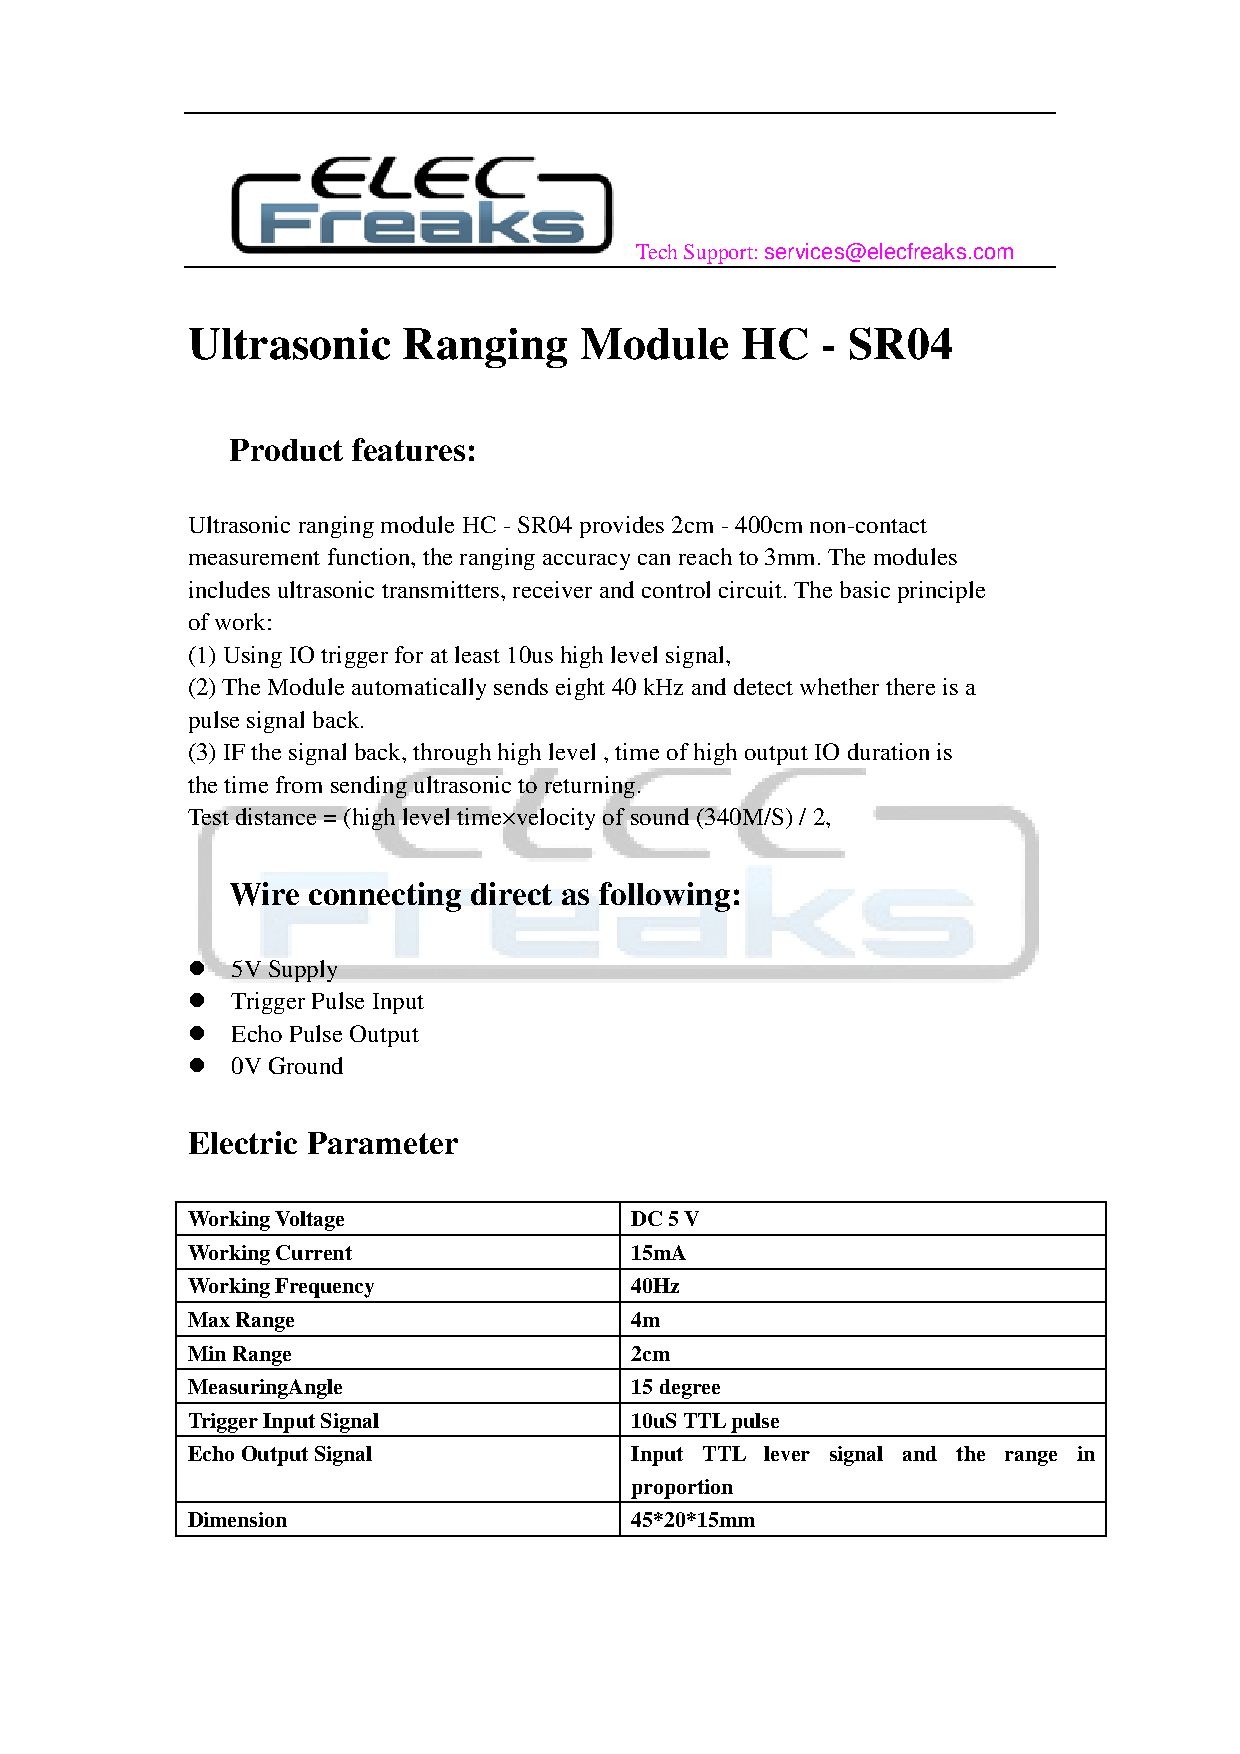
\includepdf[
pages=-,
width=1.6\textwidth,
height=1\textheight,
angle=0,
pagecommand =\section*{Ultrasonic Sensor}]{datasheets/HCSR04.pdf}


\chapter{Raspberry Pi}\label{ch:appAlabel}

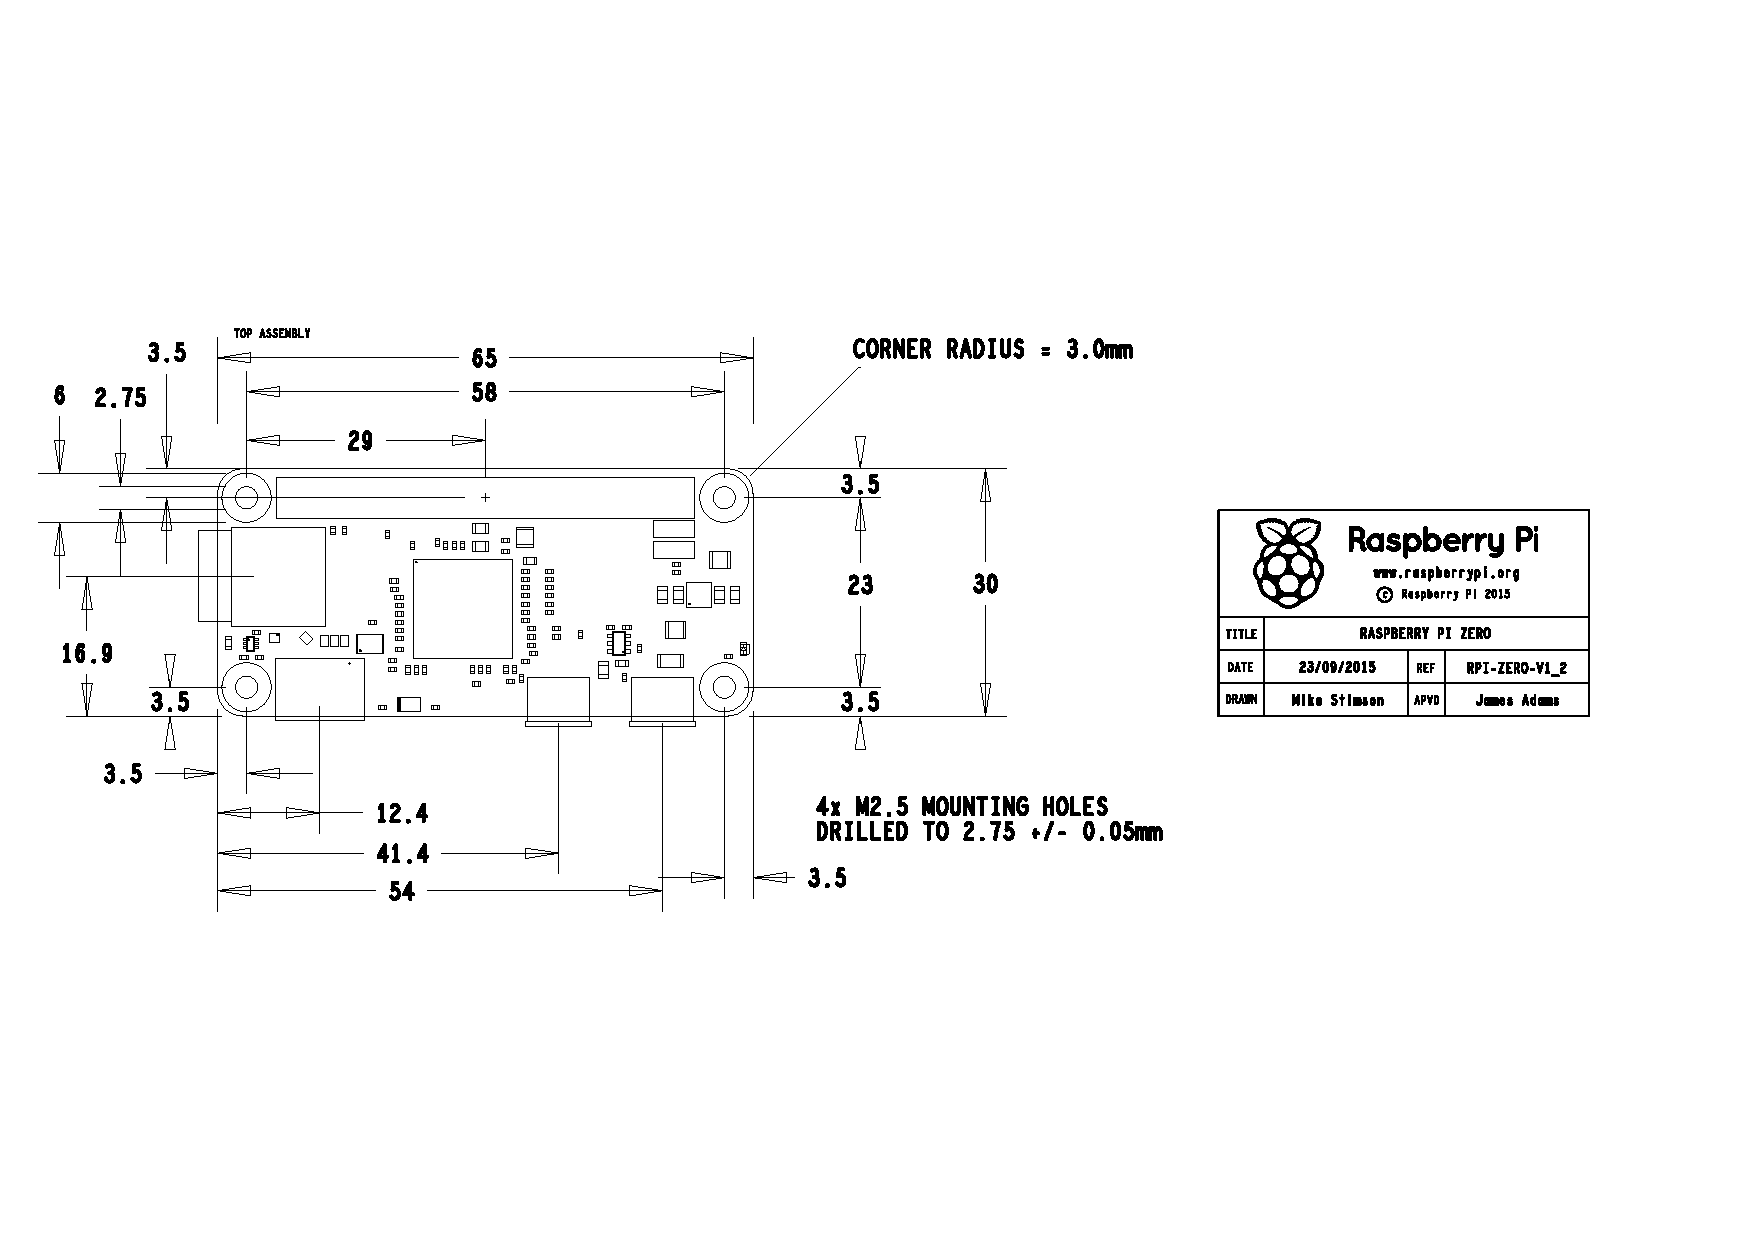
\includepdf[
pages=-,
width=1.6\textwidth,
height=1\textheight,
angle=0,
pagecommand =\section*{Raspberry Pi}]{datasheets/rpi-zero-v1_2_dimensions.pdf}

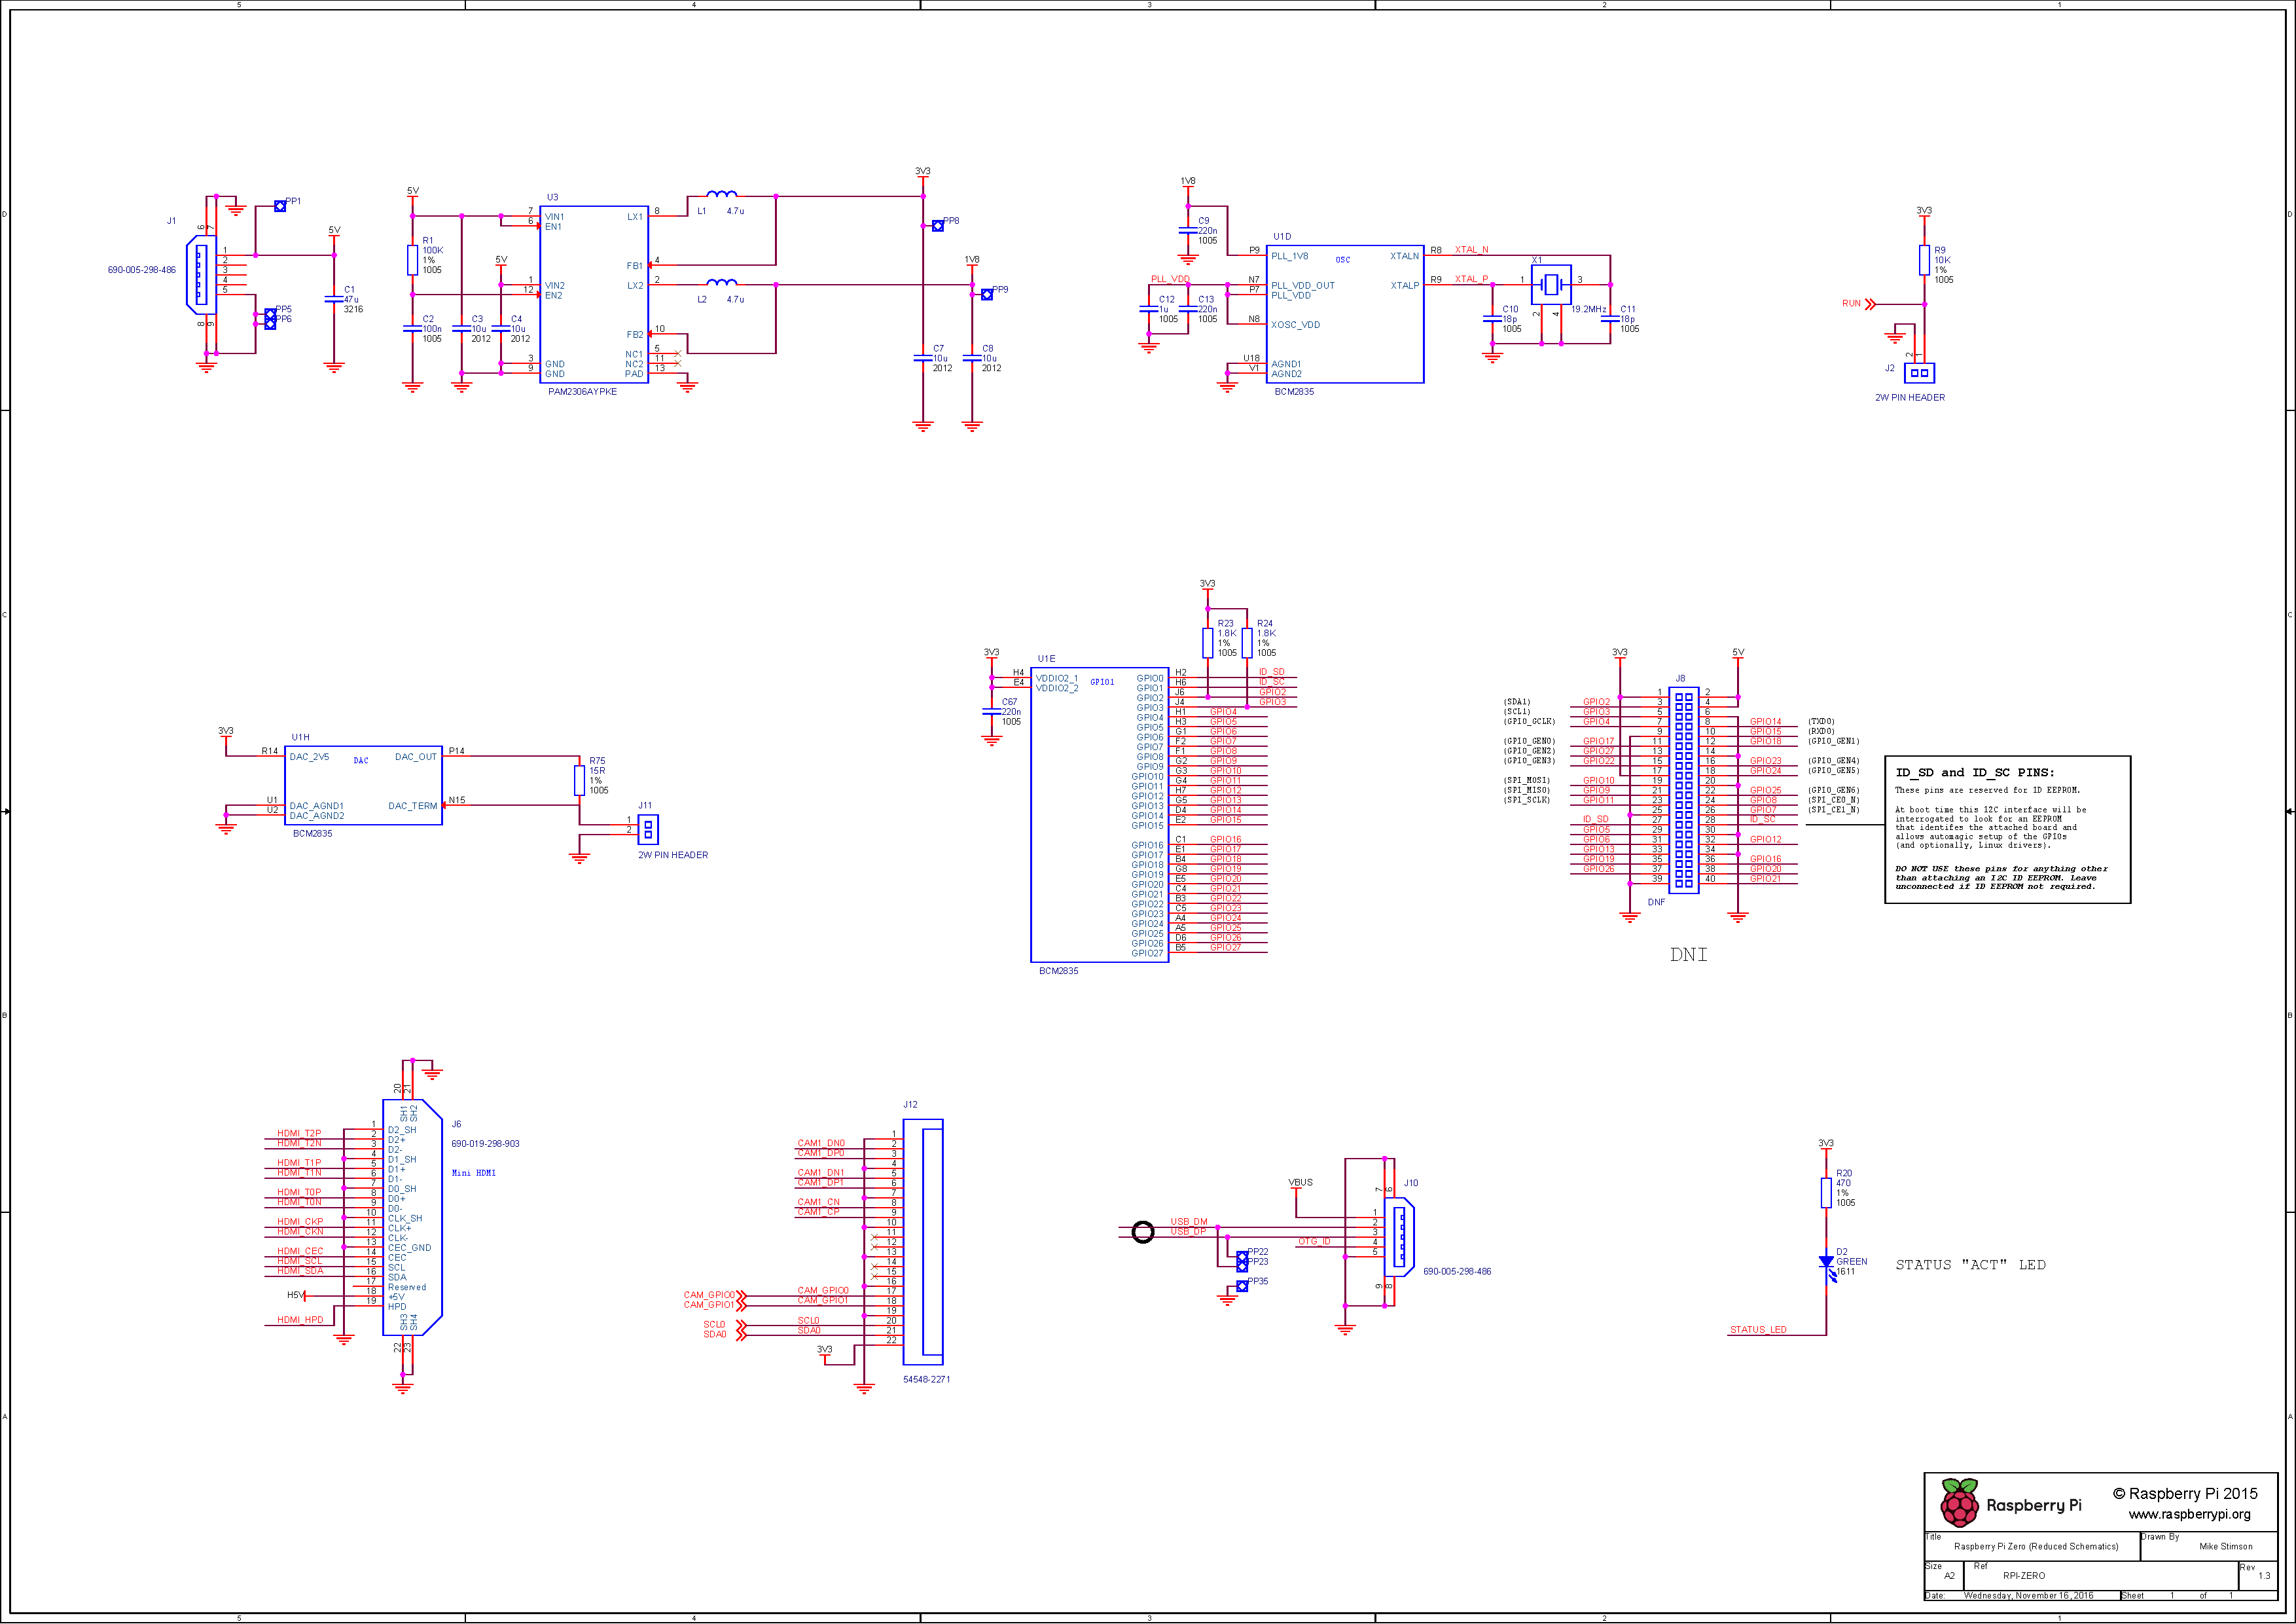
\includepdf[
pages=-,
width=1.6\textwidth,
height=1\textheight,
angle=0,
pagecommand =\section*{Raspberry Pi}]{datasheets/RPI-ZERO-V1_3_reduced.pdf}


\chapter{Source Code}\label{ch:appAlabel}

\section*{Source Code}

\begin{lstlisting}
import sys
import time
import RPi.GPIO as GPIO



#PIN numbers
LetfPWM=16
RightPWM=20
StepPinForward1=26
StepPinBackward1=19
StepPinForward2=13
StepPinBackward2=6
ECHOF=4
ECHOL=27
ECHOR=22
TRIG=17

#Values for reading the sesnsors
SPEED_OF_SOUND = 17150
measurment_count = 3
pulse = 0.00001	
pulse_duration = [0,0,0]
sensorF_data=0
sensorR_data=0
sensorL_data=0

#navigation variables
reversetime=0
turningtime = 1
MAXSPEED = 1
MEDSPEED = 0.6
MINSPEED = 0.1

#GPIO setup for each pin 
GPIO.setmode(GPIO.BCM)
GPIO.setup(StepPinForward1, GPIO.OUT)
GPIO.setup(StepPinBackward1, GPIO.OUT)
GPIO.setup(StepPinForward2, GPIO.OUT)
GPIO.setup(StepPinBackward2, GPIO.OUT)
GPIO.setup(ECHOF, GPIO.IN)
GPIO.setup(ECHOL, GPIO.IN)
GPIO.setup(ECHOR, GPIO.IN)
GPIO.setup(TRIG, GPIO.OUT)
GPIO.setup(LetfPWM, GPIO.OUT)
GPIO.setup(RightPWM, GPIO.OUT)

#PWM channels and frequency
PWML=GPIO.PWM(16, 0.5)
PWMR=GPIO.PWM(20, 0.5)

def readsensor(PIN):
	for x in range(0, 2):
		read_time_start1 = time.time()
		GPIO.output(TRIG, True)
		time.sleep(pulse)
		GPIO.output(TRIG, False)

		while GPIO.input(PIN)==0:
			pulse_start = time.time()

		while GPIO.input(PIN)==1:
			pulse_end= time.time()

		pulse_duration[x] = pulse_end - pulse_start
		time.sleep(0.05-(time.time()-read_time_start1))

	distance = sum(pulse_duration)/measurment_count* SPEED_OF_SOUND
	distance = round(distance, 2)
	print distance
	if PIN == ECHOF:
		sensorF_data=distance

	if PIN == ECHOR:
		sensorR_data=distance

	if PIN==ECHOL:
		sensorL_data=distance

def stop():
	GPIO.output(StepPinForward1, GPIO.LOW)
	GPIO.output(StepPinForward2, GPIO.LOW)
	GPIO.output(StepPinBackward1, GPIO.LOW)
	GPIO.output(StepPinBackward2, GPIO.LOW)


def reverse(reversetime,SPEED):
	print "FORWARD"
	GPIO.output(StepPinForward1, GPIO.HIGH)
	GPIO.output(StepPinForward2, GPIO.HIGH)
	PWML.start(SPEED)
	PWMR.start(SPEED)
	sleep(reversetime)
	GPIO.output(StepPinForward1, GPIO.LOW)
	GPIO.output(StepPinForward2, GPIO.LOW)

def forward(forwardtime,SPEED):
	print "REVERSE"
	GPIO.output(StepPinBackward1, GPIO.HIGH)
	GPIO.output(StepPinBackward2, GPIO.HIGH)
	PWML.start(SPEED)
	PWMR.start(SPEED)
	time.sleep(forwardtime)
	GPIO.output(StepPinBackward1, GPIO.LOW)
	GPIO.output(StepPinBackward2, GPIO.LOW)

def right(turningtime,SPEED):
	print "RIGHT"
	GPIO.output(StepPinBackward1, GPIO.HIGH)
	GPIO.output(StepPinForward2, GPIO.HIGH)
	PWML.start(SPEED)
	PWMR.start(SPEED)
	sleep(turningtime)
	GPIO.output(StepPinBackward1, GPIO.LOW)
	GPIO.output(StepPinForward2, GPIO.LOW)

def left(turningtime,SPEED):
	print "LEFT"
	GPIO.output(StepPinForward1, GPIO.HIGH)
	GPIO.output(StepPinBackward2, GPIO.HIGH)
	PWML.start(SPEED)
	PWMR.start(SPEED)
	sleep(turningtime)
	GPIO.output(StepPinForward1, GPIO.LOW)
	GPIO.output(StepPinBackward2, GPIO.LOW)

while True:
	readsensor(ECHOF)

	if sensorF_data>200:
		forward(MAXSPEED)
		
	if 200>sensorF_data>100:
		forward(MEDSPEED)

	if 100>sensorF_data>20:
		forward(MINSPEED)

	if 20>sensorF_data:
		stop()
		readsensor(ECHOR)
		readsensor(ECHOL)

		while sensorR_data<15 and sensorL_data<15:	
			reverse(MINSPEED)
			readsensor(ECHOR)
			readsensor(ECHOL)
			
		if sensorR_data>sensorL_data== True:
			right(1,MINSPEED)
			break
			
		if sensorL_data>sensorR_data==True:
			left(1,MINSPEED)
			break
			
\end{lstlisting}
\chapter{Schematics}\label{ch:appAlabel}

\begin{sidewaysfigure}
     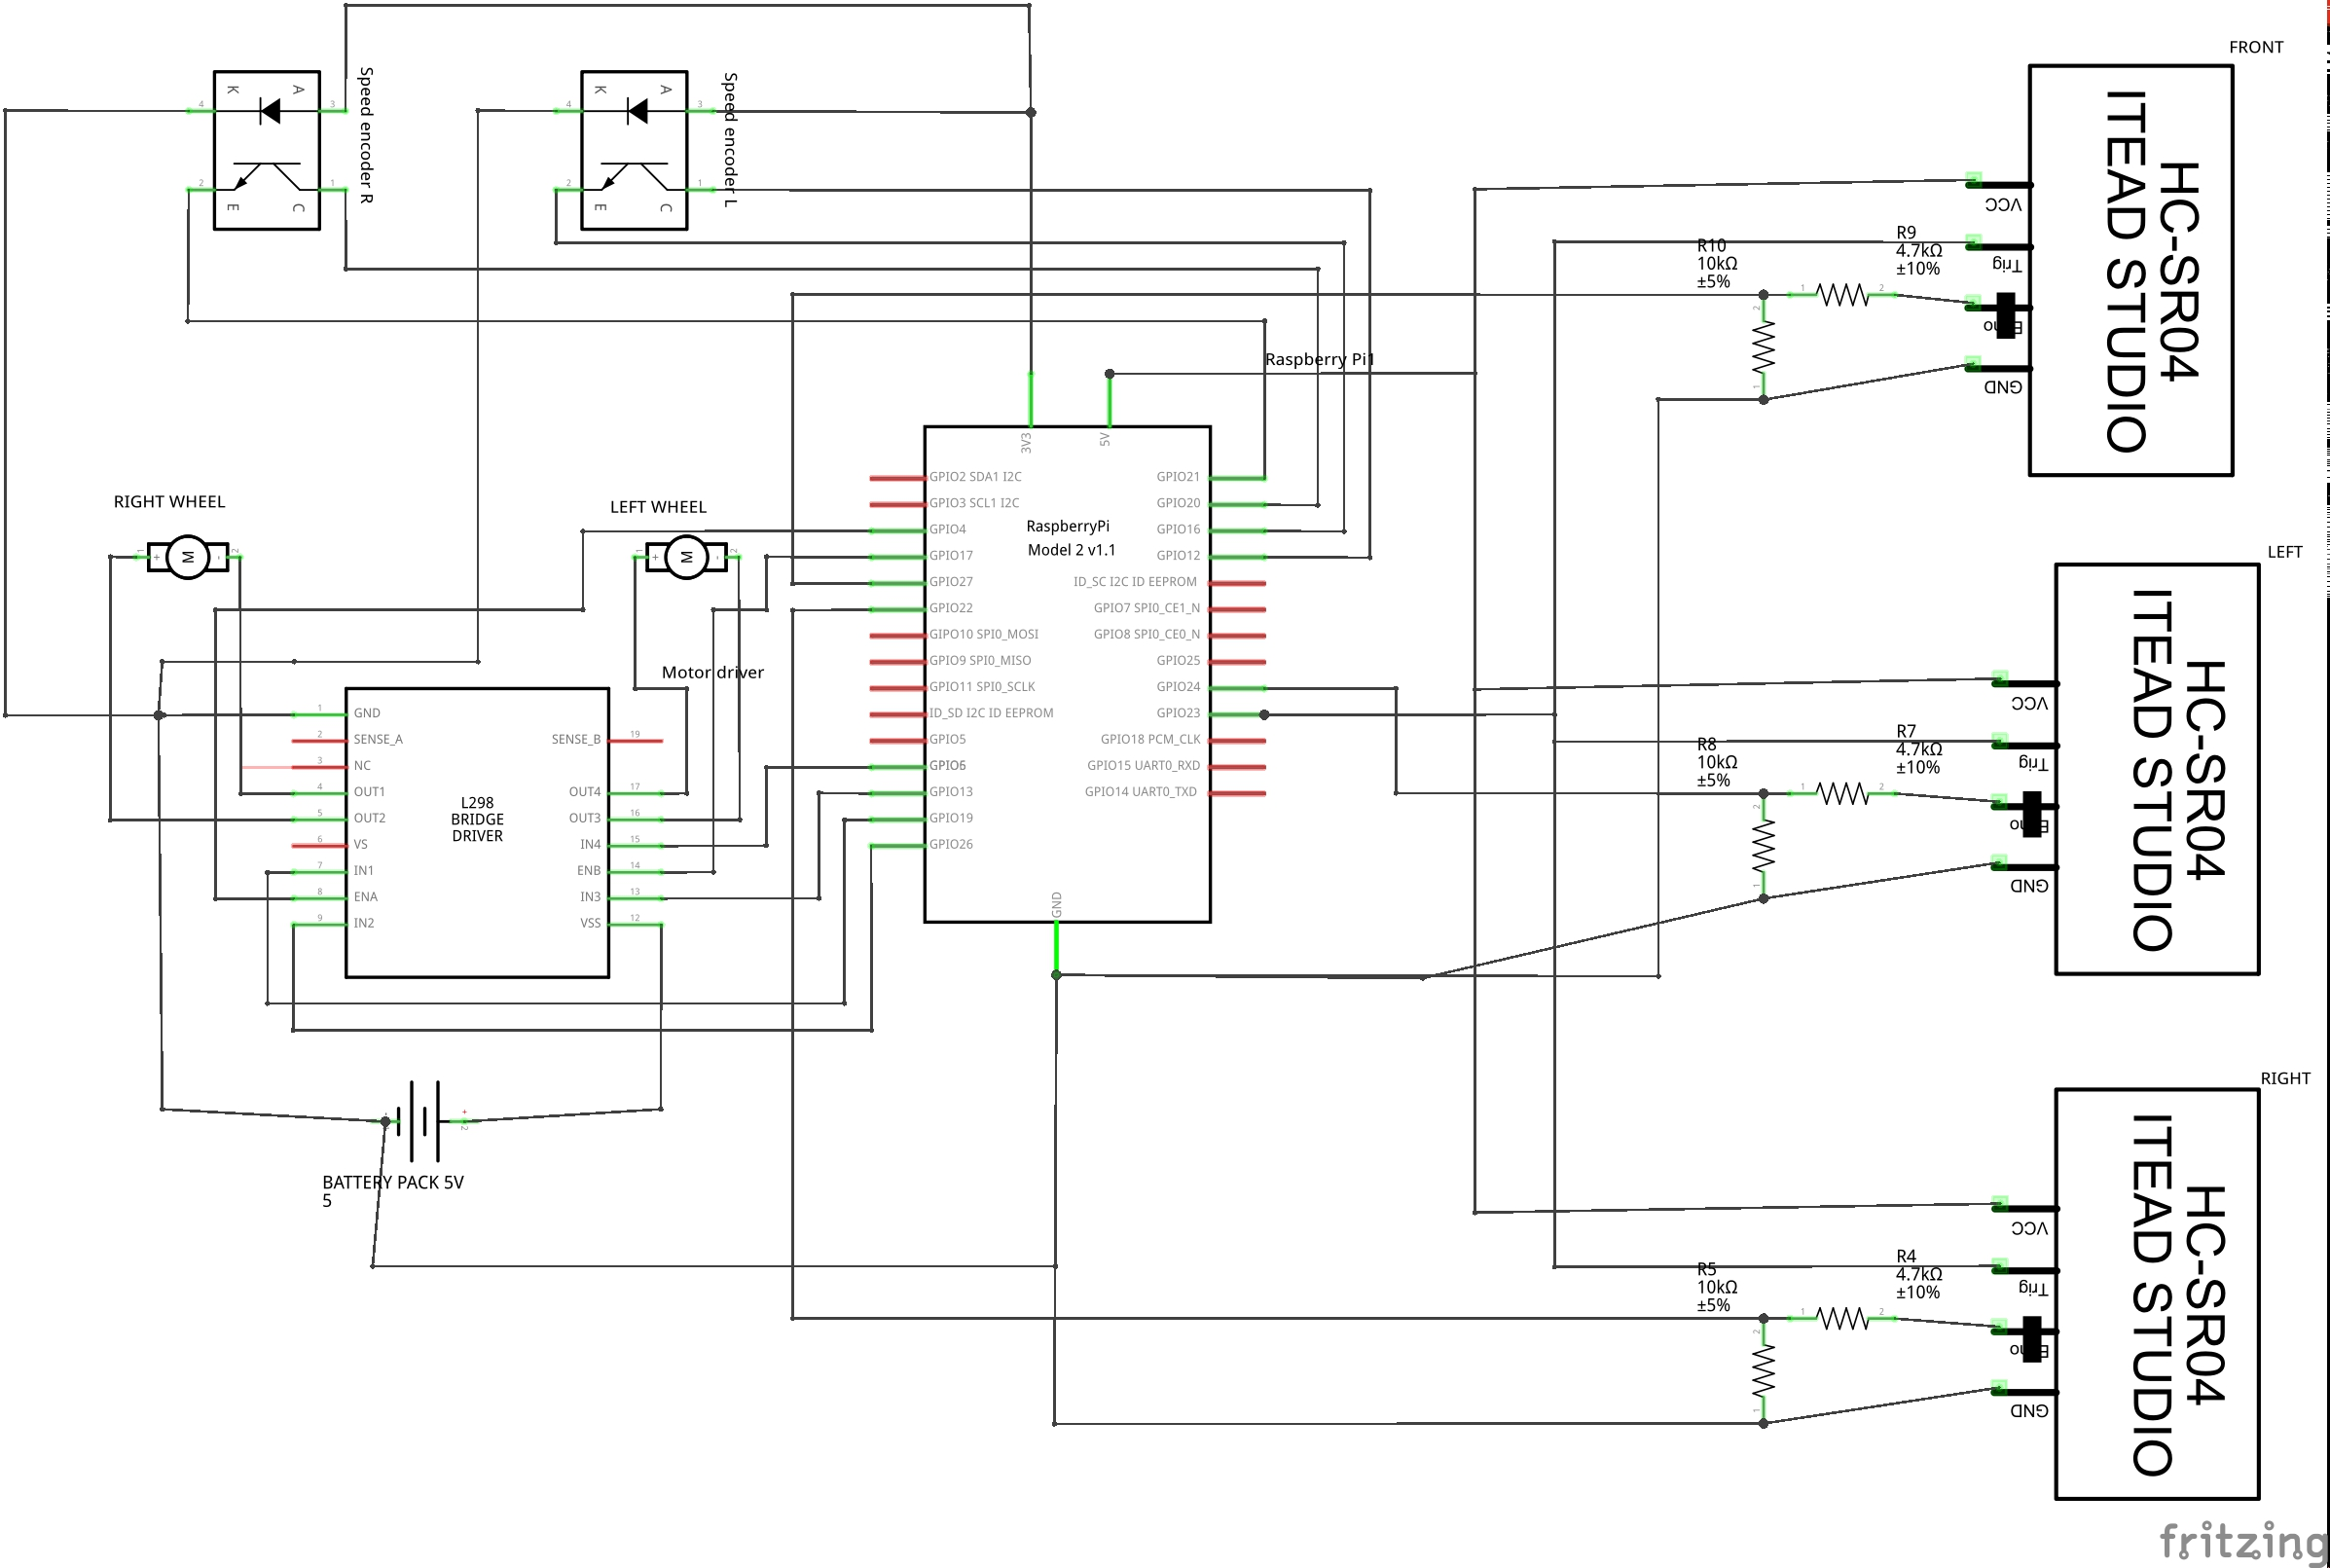
\includegraphics{P51_schem}
\end{sidewaysfigure}


\end{document}
